\documentclass[a4paper,14pt,oneside,openany]{memoir}

%%% Задаем поля, отступы и межстрочный интервал %%%

\usepackage[left=30mm, right=15mm, top=20mm, bottom=20mm]{geometry}
\pagestyle{plain}
\parindent=1.25cm
\usepackage{indentfirst}

%%% Задаем языковые параметры и шрифт %%%

\usepackage{iftex}
\ifluatex
    \usepackage{fontspec}
    \defaultfontfeatures{Ligatures=TeX}
    \setmainfont{Times New Roman}
    \setsansfont{Arial}
    \setmonofont{Courier New}
\fi
\usepackage[english, russian]{babel}

%%% Задаем стиль заголовков и подзаголовков в тексте %%%

\setsecnumdepth{subsection}
\renewcommand*{\chapterheadstart}{}
\renewcommand*{\printchaptername}{}
\renewcommand*{\chapnumfont}{\normalfont\bfseries}
\renewcommand*{\afterchapternum}{\hspace{1em}}
\renewcommand*{\printchaptertitle}{\normalfont\bfseries\centering\MakeUppercase}
\setbeforesecskip{20pt}
\setaftersecskip{20pt}
\setsecheadstyle{\raggedright\normalfont\bfseries}
\setbeforesubsecskip{20pt}
\setaftersubsecskip{20pt}
\setsubsecheadstyle{\raggedright\normalfont\bfseries}

%%% Задаем параметры оглавления %%%

\addto\captionsrussian{\renewcommand\contentsname{Содержание}}
\setrmarg{2.55em plus1fil}
\renewcommand{\aftertoctitle}{\afterchaptertitle \vspace{-\cftbeforechapterskip}}
\renewcommand*{\cftchapternumwidth}{1.5em}
\renewcommand*{\cftchapterfont}{\normalfont\MakeUppercase}
\renewcommand*{\cftchapterpagefont}{\normalfont}
\renewcommand*{\cftchapterdotsep}{\cftdotsep}
\renewcommand*{\cftdotsep}{1}
\renewcommand*{\cftchapterleader}{\cftdotfill{\cftchapterdotsep}}
\maxtocdepth{subsection}

%%% Выравнивание и переносы %%%

\tolerance 1414
\hbadness 1414
\emergencystretch 1.5em
\hfuzz 0.3pt
\vfuzz \hfuzz
\clubpenalty=10000
\widowpenalty=10000
\brokenpenalty=4991

%%% Буквы для перечислений по ГОСТ %%%

\makeatletter
    \def\russian@Alph#1{\ifcase#1\or
       А\or Б\or В\or Г\or Д\or Е\or Ж\or
       И\or К\or Л\or М\or Н\or
       П\or Р\or С\or Т\or У\or Ф\or Х\or
       Ц\or Ш\or Щ\or Э\or Ю\or Я\else\xpg@ill@value{#1}{russian@Alph}\fi}
    \def\russian@alph#1{\ifcase#1\or
       а\or б\or в\or г\or д\or е\or ж\or
       и\or к\or л\or м\or н\or
       п\or р\or с\or т\or у\or ф\or х\or
       ц\or ш\or щ\or э\or ю\or я\else\xpg@ill@value{#1}{russian@alph}\fi}
\makeatother

%%% Задаем параметры оформления рисунков и таблиц %%%

\usepackage{graphicx, caption, subcaption}
\graphicspath{{images/}}
\captionsetup[figure]{font=small, width=\textwidth, name=Рисунок, justification=centering}
\captionsetup[subfigure]{font=small}
\captionsetup[table]{singlelinecheck=false,font=small,width=\textwidth,justification=justified}
\captiondelim{ -- }
\setkeys{Gin}{width=\textwidth}
\renewcommand{\thesubfigure}{\asbuk{subfigure}}
\usepackage[section]{placeins}

%%% Задаем параметры ссылок и гиперссылок %%%

\usepackage{hyperref}
\hypersetup{
    colorlinks=true,
    linktoc=all,
    linktocpage=true,
    linkcolor=red,
    citecolor=red
}

%%% Настраиваем отображение списков %%%

\usepackage{enumitem}
\renewcommand*{\labelitemi}{\normalfont{--}}
\makeatletter
    \AddEnumerateCounter{\asbuk}{\russian@alph}
\makeatother
\renewcommand{\labelenumii}{\asbuk{enumii})}
\renewcommand{\labelenumiii}{\arabic{enumiii})}
\setlist{noitemsep, leftmargin=*}
\setlist[1]{labelindent=\parindent}
\setlist[2]{leftmargin=\parindent}
\setlist[3]{leftmargin=\parindent}

%%% Счетчики для нумерации объектов %%%

\counterwithout{figure}{chapter}
\counterwithout{equation}{chapter}
\counterwithout{table}{chapter}

%%% Реализация библиографии %%%

\usepackage{csquotes}
\usepackage[%
backend=biber,
bibencoding=utf8,
sorting=none,
style=gost-numeric,
language=auto,
autolang=other,
sortcites=true,
movenames=false,
maxnames=5,
minnames=3,
doi=false,
isbn=false,
]{biblatex}[2016/09/17]
\DeclareDelimFormat{bibinitdelim}{}
\addbibresource{biba.bib}
\defbibheading{bibliography}[\bibname]{\chapter*{#1}\addcontentsline{toc}{chapter}{#1}}

\DeclareSourcemap{
  \maps[datatype=bibtex]{
    \map{
        \step[fieldsource=title, match=\regexp{^\P{Cyrillic}*\p{Cyrillic}.*}, final]
        \step[fieldset=langid, fieldvalue={russian}]
    }
    \map{
        \step[fieldset=langid, fieldvalue={english}]
    }
  }
}

%%% Прочие пакеты %%%

\usepackage{longtable,ltcaption}
\usepackage{tabularx}
\usepackage{adjustbox}
\usepackage{multirow,makecell}
\usepackage{booktabs}
\usepackage{soulutf8}
\usepackage{icomma}
\usepackage{hyphenat}
\usepackage{textcomp}
\usepackage[version=4]{mhchem}
\usepackage{amsmath}
\usepackage{amssymb}
\usepackage{url}
\usepackage{siunitx}
\sisetup{output-decimal-marker={,}, group-separator={\,}}
\usepackage{tikz}
\usetikzlibrary{arrows.meta, positioning, fit, backgrounds, shapes.geometric, calc}
\usepackage{pgfplots}
\pgfplotsset{compat=1.18}
\usepgfplotslibrary{fillbetween}
\pgfplotsset{
  thesisplot/.style={
    width=0.92\textwidth, height=6.4cm,
    grid=major,
    grid style={gray!22, dashed},
    tick align=outside,
    tick style={gray!55},
    axis line style={gray!60},
    label style={font=\small},
    tick label style={font=\footnotesize},
    title style={font=\small\bfseries},
    legend style={font=\footnotesize, draw=gray!40, fill=white,
                  fill opacity=0.9, text opacity=1, rounded corners=1pt},
    legend cell align=left,
    every axis plot/.append style={line width=1pt},
  },
}
\usepackage{lastpage}
\usepackage{totcount}
\regtotcounter{figure}
\regtotcounter{table}
\newtotcounter{bibcnt}
\AtEveryBibitem{\stepcounter{bibcnt}}
\newcommand{\printbibcount}{\arabic{bibcnt}}

%%% Вставляем по очереди все содержательные части документа %%%

\begin{document}

% \thispagestyle{empty}

\begin{center}
    МИНИСТЕРСТВО НАУКИ И ВЫСШЕГО ОБРАЗОВАНИЯ \\ РОССИЙСКОЙ ФЕДЕРАЦИИ

    \vspace{20pt}

    Федеральное государственное автономное \\ образовательное учреждение высшего образования \\
    "<Национальный исследовательский университет ИТМО"> \\
    (Университет ИТМО)

    \vspace{20pt}

    Факультет систем управления и робототехники
\end{center}

\vfill

\begin{center}
    ВЫПУСКНАЯ КВАЛИФИКАЦИОННАЯ РАБОТА БАКАЛАВРА \\

    \vspace{20pt}

    по теме: \\
    \textbf{Исследование применения обучения с подкреплением для повышения эффективности управления роботами с использованием визуально-языковых моделей}
\end{center}

\vfill

    \noindent Студент: \\
    \textit{Группа № 3435 \hfill Д.Е. Новичков}

    \vspace{20pt}

    \noindent Руководитель ВКР: \\
    \textit{доцент ФСУиР, кандидат технических наук, \hfill А.А. Ведяков} \\
    \textit{ординарный доцент}

\vfill

\begin{center}
    Санкт-Петербург 2026
\end{center}


% \thispagestyle{empty}

\begin{center}
    \textbf{АННОТАЦИЯ}
\end{center}

\vspace{10pt}

\noindent\textbf{Студент:} Новичков Дмитрий Евгеньевич, группа~3435.

\noindent\textbf{Руководитель ВКР:} Ведяков Алексей Александрович, доцент ФСУиР, к.т.н., ординарный доцент.

\noindent\textbf{Наименование темы:} Исследование применения обучения с подкреплением для повышения эффективности управления роботами с использованием визуально-языковых моделей.

\noindent\textbf{Кафедра/факультет:} Факультет систем управления и робототехники, Университет ИТМО.

\noindent\textbf{Год защиты:} 2026.

\vspace{8pt}
\noindent\rule{\textwidth}{0.4pt}
\vspace{4pt}

\noindent\textbf{Цель исследования.}
Повышение эффективности управления роботами-манипуляторами при выполнении задач, заданных на естественном языке, за счёт интеграции методов обучения с подкреплением (RL) с визуально-языковыми моделями действий (VLA).

\vspace{6pt}
\noindent\textbf{Решаемые задачи.}
\begin{enumerate}[noitemsep, topsep=2pt]
    \item Провести аналитический обзор современных VLA-моделей и способов их интеграции с RL по работам 2023--2026~гг.\ (RT-2, OpenVLA, $\pi_0$, FLOWER, Gemini Robotics~1.5, EUREKA, RL-VLM-F, STARE-VLA, PLD и др.).
    \item Систематизировать подходы по трём направлениям: RL-дообучение VLA (Residual RL, PLD, STARE-VLA); VLM как генератор вознаграждений (EUREKA, Text2Reward, RL-VLM-F, RoboReward); VLM как высокоуровневый планировщик в связке с RL (SayCan, Embodied-R1).
    \item Разработать методику эксперимента: варьируемые факторы (алгоритм RL, способ генерации награды, архитектура и размер VLM/VLA), фиксируемые параметры, план, метрики и процедуру статистической обработки.
    \item Реализовать программный прототип (RL-дообучение VLA и модуль VLM-генерации вознаграждений) в среде симуляции.
    \item Провести экспериментальное сравнение на стандартных бенчмарках (LIBERO, MetaWorld) с базовыми методами в соответствии с разработанной методикой.
    \item Проанализировать результаты, выявить ограничения и сформулировать рекомендации по выбору архитектуры интеграции VLM+RL.
\end{enumerate}

\vspace{6pt}
\noindent\textbf{Краткая характеристика полученных результатов.}

Реализован прототип с двумя ветками: (1)~основная -- RL-дообучение VLA (residual SAC + стадийное вознаграждение) на LIBERO; (2)~дополнительная -- VLM-кодогенерация награды на MetaWorld.

\textbf{Основной результат} (серии~1--4, около 70 запусков, девять VLA-моделей, 3 seed, 95\% ДИ): OpenVLA-OFT-7B, UniVLA-7B, $\pi_0$-3B, CogACT-8B, SmolVLA-2.2B, $\pi_0$-fast-3B, SpatialVLA-4B, Octo-Small, RT-1-X. После residual SAC + stage RL прирост SR составил от +1,5~п.п.\ (OpenVLA-OFT: 97,1\% $\to$ 98,6\% $\pm$0,3) до +4,1~п.п.\ (RT-1-X: 82,9\% $\to$ 87,0\%); промежуточные: UniVLA 95,0$\to$96,8, $\pi_0$ 94,0$\to$96,1, CogACT 93,0$\to$95,4, SmolVLA 92,5$\to$95,3, $\pi_0$-fast 90,6$\to$93,8, SpatialVLA 88,0$\to$91,5, Octo 86,0$\to$89,9. Установлена сильная обратная корреляция ($\rho = -0{,}97$) между baseline SR и приростом. End-to-end разморозка VLA деградирует ($-$0,6~п.п.). Стадийное вознаграждение даёт +0,8~п.п.\ над разреженным. Результат 98,6\% сопоставим с PLD (99,0\% на LIBERO) при бюджете в 3 раза меньше.

\textbf{Дополнительный результат} (серия~5, MetaWorld): VLM-награда с 3 итерациями рефлексии поднимает SR на push-v3 с 48\% до 85\% ($\rho(R,S)$: 0,12 $\to$ 0,81); средний SR по трём задачам -- 77,2\% (vs 36,7\% у разреженной награды).

Сформулированы 5 рекомендаций по выбору архитектуры интеграции VLM+RL: при наличии предобученной VLA (SR\,$>$\,90\%) -- residual RL с замороженной базой и стадийной наградой; при отсутствии VLA -- VLM-генерация награды с итеративным уточнением; SAC предпочтительнее PPO в residual-постановке. Прототип реализован с открытым исходным кодом (\url{https://github.com/mfclabber/bachelor-thesis}).

\vspace{6pt}
\noindent\textbf{Ключевые слова:} обучение с подкреплением, визуально-языковые модели действий, residual RL, VLM-генерация вознаграждений, LIBERO, MetaWorld, OpenVLA, стадийное вознаграждение, робототехническое манипулирование.

\vspace{6pt}
\noindent\rule{\textwidth}{0.4pt}

\vspace{6pt}
\noindent\textbf{Объём работы:} \pageref{LastPage}~страниц, \ref{fig:last}~рисунков, \ref{tab:last}~таблиц, \printbibcount~источника.

\clearpage


\setcounter{page}{6}
\OnehalfSpacing*

\tableofcontents*

\chapter*{Список сокращений и обозначений}
\addcontentsline{toc}{chapter}{Список сокращений и обозначений}
\label{ch:abbreviations}

\begin{description}[
    style=nextline,
    leftmargin=2.2cm,
    labelwidth=1.6cm,
    labelsep=0.4cm,
    font=\normalfont\bfseries,
    itemsep=0.15cm
]
    \item[BC]   Behavioral Cloning (обучение методом поведенческого клонирования)
    \item[CLIP] Contrastive Language--Image Pre-training
    \item[DoF]  Degrees of Freedom (степени свободы)
    \item[DPO]  Direct Preference Optimization
    \item[FAST] Frequency-space Action Sequence Tokenization (частотная токенизация действий)
    \item[GRPO] Group Relative Policy Optimization
    \item[LLM]  Large Language Model (большая языковая модель)
    \item[LoRA] Low-Rank Adaptation (низкоранговая адаптация)
    \item[LOOP] Leave-One-Out PPO (безкритиковая схема RL)
    \item[MDP]  Markov Decision Process (марковский процесс принятия решений)
    \item[MLP]  Multilayer Perceptron (многослойный перцептрон)
    \item[OFT]  Optimized Fine-Tuning (оптимизированный рецепт дообучения OpenVLA)
    \item[OXE]  Open X-Embodiment (набор робототехнических данных)
    \item[PPO]  Proximal Policy Optimization
    \item[RL]   Reinforcement Learning (обучение с подкреплением)
    \item[RLOO] REINFORCE Leave-One-Out
    \item[SAC]  Soft Actor-Critic
    \item[SFT]  Supervised Fine-Tuning (дообучение с учителем)
    \item[SOTA] State of the Art (наилучший достигнутый результат)
    \item[SR]   Success Rate (доля успешных выполнений)
    \item[VLA]  Vision-Language-Action (визуально-языковая модель действий)
    \item[VLM]  Vision-Language Model (визуально-языковая модель)
    \item[ДИ]   Доверительный интервал
\end{description}

\endinput


\chapter*{Введение}
\addcontentsline{toc}{chapter}{Введение}
\label{ch:intro}

    Управление робототехническими системами по инструкциям на естественном языке является одной из центральных задач современной робототехники. За последние три года в этой области произошёл качественный сдвиг благодаря появлению визуально-языковых моделей действий (Vision-Language-Action, VLA) -- класса моделей, объединяющих визуальное восприятие, понимание языка и генерацию управляющих команд в единой архитектуре \cite{brohan2023rt2, kim2024openvla, black2024pi0}. Модели этого класса обучаются на крупномасштабных визуально-языковых данных из Интернета и дообучаются на робототехнических демонстрациях, что позволяет им следовать произвольным текстовым инструкциям и обобщать на новые объекты и среды.

    Интерес к VLA-моделям демонстрирует взрывной рост: по данным поиска на платформе OpenReview по ключевому слову <<Vision-Language-Action>>, на конференции ICLR 2024 была подана лишь одна такая работа, на ICLR 2025 -- девять, а к ICLR 2026 их число достигло 164, что соответствует примерно восемнадцатикратному росту всего за год \cite{reuss2025blog} (рисунок~\ref{fig:vla_growth}). Ключевыми представителями данного направления являются RT-2 \cite{brohan2023rt2} с 55 миллиардами параметров, показавший двукратное превосходство над предшественником на новых объектах; OpenVLA \cite{kim2024openvla} -- открытая модель с 7 миллиардами параметров, превосходящая RT-2-X на 16,5\% по метрике успешности; $\pi_0$ \cite{black2024pi0} от Physical Intelligence, использующая flow matching для генерации действий; и FLOWER \cite{reuss2025flower} -- компактная модель с 950 миллионами параметров, достигшая state-of-the-art на бенчмарке CALVIN.

\begin{figure}[htbp]
    \centering
    \begin{tikzpicture}
        \begin{axis}[
            thesisplot,
            ybar,
            bar width=26pt,
            height=5.6cm, width=0.66\textwidth,
            ylabel={Число работ по VLA},
            symbolic x coords={ICLR 2024, ICLR 2025, ICLR 2026},
            xtick=data,
            ymin=0, ymax=185,
            nodes near coords,
            nodes near coords style={font=\footnotesize},
            enlarge x limits=0.28,
        ]
        \addplot[fill=blue!45, draw=blue!60!black] coordinates {(ICLR 2024,1) (ICLR 2025,9) (ICLR 2026,164)};
        \end{axis}
    \end{tikzpicture}
    \caption{Рост числа работ по тематике Vision-Language-Action на ICLR (поиск по ключевому слову на OpenReview, по данным~\cite{reuss2025blog}).}
    \label{fig:vla_growth}
\end{figure}

    Однако, несмотря на впечатляющий прогресс, успешность выполнения операций VLA-моделями в реальных условиях остаётся на уровне 70--80\%, что недостаточно для надёжного практического применения \cite{reuss2025blog}. Между открытыми моделями и закрытыми фронтирными системами, такими как Gemini Robotics 1.5 \cite{deepmind2025gemini}, существует значительный разрыв в способности к zero-shot обобщению, который не виден из результатов на стандартных бенчмарках. Обучение с подкреплением (Reinforcement Learning, RL) рассматривается как одно из ключевых направлений преодоления этого разрыва. RL позволяет агенту улучшать политику управления через взаимодействие со средой на основе сигнала вознаграждения, что потенциально может довести успешность VLA-моделей с 70--80\% до требуемых 99\%+.

    Интеграция RL и визуально-языковых моделей развивается по нескольким направлениям. Первое -- RL-дообучение уже обученных VLA-моделей: работы PLD \cite{pld2026} (99\% на LIBERO) и stage-aware RL \cite{starevla2025} (98\% на SIMPLER), представленные на ICLR 2026, показывают, что residual RL и стадийные вознаграждения позволяют почти полностью закрыть разрыв на стандартных бенчмарках. Второе -- использование визуально-языковых моделей для автоматической генерации функций вознаграждения, заменяющих трудоёмкое ручное проектирование наград: EUREKA \cite{ma2024eureka} превосходит экспертные вознаграждения на 83\% задач, а Text2Reward \cite{xie2024text2reward} генерирует плотные reward-функции в виде исполняемого кода, не уступая экспертным на 13 из 17 задач. Третье -- применение VLM в качестве высокоуровневого планировщика в связке с RL-агентом \cite{ahn2022saycan, embodiedr1_2026}. Тем не менее, ни один из методов интеграции RL и VLA пока не утвердился как стандартный подход -- эта проблема остаётся открытой.

    \textbf{Объект исследования} -- процессы обучения и дообучения визуально-языковых моделей действий для робототехнического манипулирования с применением обучения с подкреплением.

    \textbf{Предмет исследования} -- методы RL-дообучения визуально-языковых моделей действий (residual RL, стадийные вознаграждения, заморозка базовой политики), закономерности прироста SR в зависимости от baseline-качества VLA, а также сравнительная эффективность VLM-генерации наград как альтернативного направления интеграции.

    \textbf{Актуальность.} Несмотря на высокие результаты VLA-моделей в симуляции (до 99\% на LIBERO), их надёжность в реальных условиях остаётся недостаточной. RL рассматривается как ключевой инструмент доведения SR до промышленно приемлемого уровня, однако отсутствует единая методика выбора схемы интеграции VLM/VLA и RL с учётом доступных данных и вычислительных ресурсов.

    \textbf{Научная новизна} работы состоит в следующем:
    \begin{enumerate}
        \item предложена единая классификация подходов интеграции RL и VLM/VLA по восьми критериям с количественным сопоставлением результатов из литературы;
        \item экспериментально сравнены девять открытых VLA-моделей (OpenVLA-OFT, UniVLA, $\pi_0$, CogACT, SmolVLA, $\pi_0$-fast, SpatialVLA, Octo, RT-1-X) на бенчмарке LIBERO в едином протоколе до и после RL-дообучения;
        \item установлено, что residual SAC со стадийным вознаграждением стабильно повышает SR на 1,5--4,1~п.п., тогда как end-to-end разморозка VLA приводит к деградации ($-$0,6~п.п.);
        \item показана закономерность: наибольший прирост от RL получают модели с более низким baseline SR (RT-1-X: +4,1~п.п.), наименьший -- у лидеров (OpenVLA: +1,5~п.п.);
        \item в дополнительной серии на MetaWorld подтверждено, что VLM-награды при 3 итерациях рефлексии поднимают SR на контактной задаче push-v3 с 48\% до 85\%.
    \end{enumerate}

    \textbf{Практическая значимость.} Основной результат -- выбор VLA и схемы RL-дообучения (residual SAC + стадийное вознаграждение при SR\,$>$\,90\%). Дополнительная серия VLM-наград покрывает сценарий без VLA (рисунок~\ref{fig:decision_tree}).

    Целью настоящей работы является разработка методических рекомендаций по применению обучения с подкреплением в задачах обучения и дообучения визуально-языковых моделей действий для робототехнического манипулирования. Для достижения цели поставлены следующие задачи:

\begin{enumerate}
    \item Провести аналитический обзор современных VLA-моделей и способов их интеграции с обучением с подкреплением на основе работ 2022--2026 гг.
    \item Систематизировать и классифицировать существующие подходы по трём направлениям: RL-дообучение VLA, VLM-генерация вознаграждений для RL, VLM как планировщик в связке с RL.
    \item Разработать методику проведения вычислительного эксперимента.
    \item Реализовать программный прототип RL-дообучения VLA и дополнительный модуль VLM-генерации наград в среде симуляции.
    \item Провести экспериментальное сравнение на стандартных бенчмарках с базовыми методами.
    \item Проанализировать результаты, выявить ограничения и сформулировать рекомендации по выбору архитектуры интеграции VLM и RL.
\end{enumerate}

    Работа организована следующим образом. В главе~\ref{ch:chap1} приведён аналитический обзор VLA-моделей, методов RL и подходов к их интеграции. В главе~\ref{ch:chap2} сформулирована постановка задачи, обоснован выбор RL-дообучения VLA, описана архитектура residual RL и методика эксперимента. В главе~\ref{ch:chap3} описана реализация прототипа: основные серии~1--4 (VLA+RL, LIBERO) и дополнительная серия~5 (VLM-награды, MetaWorld). В заключении сформулированы методические рекомендации.

    Центральная логика (рисунок~\ref{fig:thesis_roadmap}): \textbf{фокус} -- VLA-baseline $\to$ RL-схемы $\to$ RL всех моделей $\to$ абляция; \textbf{дополнение} -- VLM-награды на MetaWorld.

\begin{figure}[htbp]
    \centering
    \begin{tikzpicture}[
        node distance=0.85cm and 2.6cm,
        stage/.style={draw, rounded corners=2pt, align=center, text width=4.0cm, minimum height=1.0cm, font=\small},
        series/.style={draw, rounded corners=2pt, align=center, text width=4.4cm, minimum height=0.85cm, font=\small},
        line/.style={semithick},
        arr/.style={line, -{Stealth[length=3mm, width=2.2mm]}},
        dasharr/.style={line, dashed, -{Stealth[length=3mm, width=2.2mm]}}
    ]
        \node[stage, fill=green!12] (g1) {Глава 1:\\обзор VLA + RL};
        \node[stage, fill=blue!10, below=of g1] (g2) {Глава 2:\\постановка и методика};
        \node[stage, fill=orange!12, below=of g2] (g3) {Глава 3:\\VLA+RL (осн.) + VLM (доп.)};
        \node[stage, fill=purple!10, below=of g3] (g4) {Заключение:\\рекомендации};

        \draw[arr] (g1.south) -- (g2.north);
        \draw[arr] (g2.south) -- (g3.north);
        \draw[arr] (g3.south) -- (g4.north);

        \node[series, fill=gray!10, right=2.8cm of g2] (s1) {С1: VLA-baseline (9 моделей)};
        \node[series, fill=gray!10, below=0.45cm of s1] (s2) {С2: RL-схемы (OpenVLA)};
        \node[series, fill=gray!10, below=0.45cm of s2] (s3) {С3: RL всех VLA (residual SAC)};
        \node[series, fill=gray!10, below=0.45cm of s3] (s4) {С4: абляция (stage, freeze)};
        \node[series, fill=orange!10, below=0.45cm of s4] (s5) {С5: VLM-награда (MetaWorld)};

        \node[draw, dashed, rounded corners=3pt, inner sep=0.35cm, fit=(s1)(s5), label={[font=\small]above:Экспериментальные серии}] {};

        \coordinate (linkH) at ($(g3.east)+(0.9,0)$);
        \coordinate (linkV) at (linkH |- s2.west);
        \draw[line, dashed] (g3.east) -- (linkH);
        \draw[line, dashed] (linkH) -- (linkV);
        \draw[dasharr] (linkV) -- (s2.west);
    \end{tikzpicture}
    \caption{Структура работы и логика экспериментальных серий.}
    \label{fig:thesis_roadmap}
\end{figure}

\endinput

\chapter{Аналитический обзор}
\label{ch:chap1}

\section{Визуально-языковые модели действий}
\label{sec:vla}

    Визуально-языковая модель действий (Vision-Language-Action model, VLA) -- это модель, использующая предобученный backbone, обученный на крупномасштабных визуально-языковых данных из Интернета, и впоследствии дообученная на генерацию управляющих команд робота \cite{reuss2025blog}. Управляющие команды могут представлять собой углы сочленений, положение концевого эффектора, состояние захвата и другие управляющие воздействия. В отличие от мультимодальных политик, использующих раздельно предобученные текстовый и визуальный энкодеры, VLA-модели опираются на совместное визуально-языковое предобучение, что теоретически обеспечивает более глубокое понимание языковых инструкций и лучшее обобщение.

    По архитектуре генерации действий современные VLA-модели подразделяются на три основных класса.

    Авторегрессионные модели представляют действия в виде последовательности дискретных токенов и генерируют их поочерёдно, аналогично генерации текста в языковых моделях. К этому классу относится RT-2 \cite{brohan2023rt2} -- модель с 55 миллиардами параметров, дообученная на робототехнических траекториях поверх предобученной визуально-языковой модели PaLI-X. На 6000 испытаниях RT-2 продемонстрировала двукратное превосходство над RT-1 при работе с новыми объектами и средами, а также emergent-способности к chain-of-thought рассуждениям. OpenVLA \cite{kim2024openvla} -- открытая 7B модель на основе Llama~2 с объединённым визуальным энкодером DINOv2 и SigLIP. Обучена на 970~000 реальных робототехнических траекторий из набора Open X-Embodiment, охватывающих более 70 доменов задач. Превосходит RT-2-X на 16,5\% по абсолютному success rate на 29 задачах, при этом имея в 8 раз меньше параметров. Поддерживает эффективное дообучение через LoRA на потребительских GPU.

    Диффузионные и flow-matching модели генерируют непрерывные траектории действий через итеративный процесс денойзинга. Модель $\pi_0$ \cite{black2024pi0} от Physical Intelligence использует PaliGemma (3B) в качестве визуально-языкового backbone и flow matching для генерации действий. Предобучена на данных с 7 конфигураций роботов и 68 задач, код и веса доступны через репозиторий openpi; на LIBERO достигает среднего SR 94,2\% (Spatial 96,8\%, Object 98,8\%, Goal 95,8\%, Long 85,2\%). Вариант $\pi_0$-FAST \cite{black2024pi0} применяет частотное токенизирование действий (FAST) для ускорения генерации и показывает 85,5\% в среднем. FLOWER \cite{reuss2025flower} -- компактная модель с 950M параметров, достигающая state-of-the-art на CALVIN ABC (4,53) при обучении всего за 200~H100-часов. Использует intermediate-modality fusion с сокращением LLM-слоёв на 50\% и перераспределением ёмкости в диффузионную голову.

    Дискретно-диффузионные модели -- новейший класс, представленный на ICLR 2026. В отличие от авторегрессионных, они генерируют последовательности действий параллельно через дискретную диффузию, что позволяет одновременно создавать и рассуждения, и действия. К этому классу относятся Discrete Diffusion VLA, dVLA и DiVA, показывающие результаты 95--98\% на LIBERO.

\subsection{Дополнительные открытые VLA-модели}
\label{subsec:more_vla}

    Помимо базовых моделей, для экспериментального исследования (глава~\ref{ch:chap3}) привлечён ряд более новых открытых VLA, демонстрирующих конкурентные результаты на LIBERO.

    \textbf{UniVLA} \cite{univla2025} -- унифицированная мультимодальная модель, обучающая зрение, язык и действие в едином авторегрессионном пространстве дискретных токенов с включением видеоданных в обучение мира. Достигает среднего SR 95,5\% на LIBERO, причём ключевой вклад -- скачок на длинногоризонтном наборе Long с прежних 69,0\% до 94,0\%.

    \textbf{CogACT} \cite{cogact2024} -- модель, разделяющая когнитивный (VLM-рассуждение) и моторный (диффузионный action-эксперт) модули. На LIBERO показывает средний SR 93,6\% (Spatial 97,2\%, Object 98,0\%, Goal 90,2\%, Long 88,8\%), демонстрируя устойчивость на длинных задачах за счёт специализированной action-головы.

    \textbf{SpatialVLA} \cite{spatialvla2025} -- VLA с явным кодированием пространственных представлений (Ego3D position encoding, adaptive action grids), backbone 4B. Средний SR на LIBERO -- 78,1\% (Spatial 88,2\%, Object 89,9\%, Goal 78,6\%, Long 55,5\%); модель сильна в пространственном обобщении, но уступает на длинногоризонтных композиционных задачах.

    \textbf{Octo} \cite{octo2024} и \textbf{OpenVLA} \cite{kim2024openvla} в исходных (не-OFT) версиях служат нижними границами: 75,1\% и 76,5\% в среднем на LIBERO соответственно, что подчёркивает значимость рецепта дообучения OFT (parallel decoding + action chunking + L1-регрессия), поднимающего OpenVLA до 97,1\%.

\subsection{Фронтирные модели}
\label{subsec:frontier}

    Отдельного рассмотрения заслуживают закрытые фронтирные модели, определяющие верхнюю границу возможностей VLA. PaLM-E \cite{driess2023palme} -- мультимодальная языковая модель с 562 миллиардами параметров, инъецирующая непрерывные сенсорные данные в пространство эмбеддингов языковой модели. Достигла state-of-the-art на задачах визуального вопросно-ответного диалога (OK-VQA) при сохранении робототехнических способностей. Gemini Robotics 1.5 \cite{deepmind2025gemini}, представленная DeepMind в сентябре 2025 года, ввела механизм motion transfer для zero-shot переноса навыков между разными платформами роботов и <<embodied thinking>> -- чередование внутренних рассуждений на естественном языке с генерацией действий.

    Между открытыми и фронтирными моделями существует разрыв, который не виден из симуляционных бенчмарков. Открытые модели, такие как FLOWER и OpenVLA, конкурентоспособны на LIBERO и CALVIN, однако значительно уступают Gemini Robotics и $\pi_{0.5}$ по способности к zero-shot обобщению на произвольные объекты и инструкции в реальном мире \cite{reuss2025blog}. Среди причин этого разрыва -- ограниченное качество открытых данных, насыщение текущих бенчмарков и отсутствие ресурсов для масштабных реальных испытаний в академических лабораториях.

\section{Обучение с подкреплением в робототехнике}
\label{sec:rl}

    Обучение с подкреплением (Reinforcement Learning, RL) -- парадигма машинного обучения, в которой агент обучается принимать решения через взаимодействие со средой, максимизируя кумулятивный сигнал вознаграждения \cite{sutton2018rl}. В контексте робототехнического манипулирования агентом выступает робот, средой -- физическое или симулированное окружение, действиями -- управляющие команды, а состояниями -- визуальные наблюдения и проприоцептивная информация.

    Среди алгоритмов RL, наиболее широко применяемых в робототехнике, выделяются PPO (Proximal Policy Optimization) \cite{schulman2017ppo} -- on-policy алгоритм с клипированным суррогатным функционалом, обеспечивающий стабильное обучение за счёт ограничения размера обновления политики, и SAC (Soft Actor-Critic) \cite{haarnoja2018sac} -- off-policy алгоритм, максимизирующий энтропийно-регуляризованный функционал, что поощряет исследование и повышает робастность к начальным условиям. TD3 (Twin Delayed DDPG) \cite{fujimoto2018td3} решает проблему переоценки Q-функции через использование двух критиков и задержанного обновления политики.

    Ключевым узким местом применения RL в робототехнике является проектирование функции вознаграждения (reward engineering). Определение информативного вознаграждения для сложных манипуляционных задач требует экспертных знаний и трудоёмкой итеративной настройки. Разреженные вознаграждения (бинарный сигнал <<задача выполнена / не выполнена>>) приводят к крайне медленному обучению, а плотные вознаграждения сложно проектировать для произвольных задач без формализации промежуточных подцелей. Эта проблема мотивирует использование визуально-языковых моделей для автоматизации проектирования вознаграждений.

\section{Интеграция RL и визуально-языковых моделей}
\label{sec:integration}

    По результатам анализа литературы выделяются три основных направления интеграции обучения с подкреплением и визуально-языковых моделей в задачах робототехнического манипулирования.

\subsection{Классификация подходов интеграции}
\label{subsec:integration-classification}

    Для систематизации работ введём классификацию по трём направлениям: (1) RL-дообучение VLA (policy fine-tuning), (2) VLM как генератор функции вознаграждения (reward generation), (3) VLM как планировщик/декомпозитор в связке с RL (planning + skills/RL). Сводная классификация приведена в таблице~\ref{tab:integration-classification}.

\begingroup
\setlength{\tabcolsep}{3pt}
\renewcommand{\arraystretch}{1.2}
\footnotesize
\begin{longtable}{>{\raggedright\arraybackslash}p{0.17\textwidth} >{\raggedright\arraybackslash}p{0.26\textwidth} >{\raggedright\arraybackslash}p{0.26\textwidth} >{\raggedright\arraybackslash}p{0.25\textwidth}}
\caption{Классификация подходов интеграции VLM/VLA и RL.}
\label{tab:integration-classification}\\
\toprule
\textbf{Аспект} & \makecell[l]{\textbf{RL-дообучение}\\\textbf{VLA}} & \makecell[l]{\textbf{VLM $\rightarrow$ награда}\\\textbf{$\rightarrow$ RL}} & \makecell[l]{\textbf{VLM-планирование}\\\textbf{+ RL/навыки}} \\
\midrule
\endfirsthead
\toprule
\textbf{Аспект} & \makecell[l]{\textbf{RL-дообучение}\\\textbf{VLA}} & \makecell[l]{\textbf{VLM $\rightarrow$ награда}\\\textbf{$\rightarrow$ RL}} & \makecell[l]{\textbf{VLM-планирование}\\\textbf{+ RL/навыки}} \\
\midrule
\endhead
\midrule
\multicolumn{4}{r}{\small Продолжение на следующей странице} \\
\endfoot
\bottomrule
\endlastfoot
\textbf{Постановка задачи} &
Улучшить готовую политику $\pi_{\text{VLA}}(a|o,l)$, повысив SR за счёт онлайнового взаимодействия (часто через residual-обёртку) &
Снять зависимость от ручной награды, сгенерировать $R_{\text{VLM}}$ из языка/видео и обучить RL-агента &
Решать длинногоризонтные задачи: VLM выбирает/синтезирует высокоуровневые подцели/планы, низкий уровень исполняется RL/навыками \\
\textbf{Модальности} &
Зрение + язык $\rightarrow$ действия; для RL-части обычно состояния/фичи среды + (иногда) визуальные наблюдения &
Зрение (кадры/рендеры) + язык (инструкция/описание цели); опционально состояние симулятора для кодогенерации &
Зрение + язык; дополнительно список навыков/примитивов, карты сцены, API среды \\
\textbf{Роль RL} &
Основной механизм улучшения политики (онлайн дообучение, residual RL, предпочтения/стадии) &
Основной механизм обучения политики при автоматически получаемой награде (код/оценка/предпочтения) &
Компонент низкоуровневого управления (навыки/контроллеры) и/или оценка выполнимости действий (affordance/value) \\
\textbf{Тип данных} &
Демонстрации для начального SFT/BC + онлайновые траектории (симуляция и/или реальность); иногда предпочтения по стадиям &
Описания задач + (часто) доступ к коду среды/состоянию + траектории RL; данные для обучения reward-модели (если есть) &
Данные для VLM (общее предобучение) + навыковые датасеты/трейсы; иногда интерактивные данные для уточнения планов \\
\textbf{Типовые метрики} &
SR/episode success, recovery success, обобщение на новые объекты/инструкции, робастность; иногда cost/latency &
SR и reward, sample efficiency (шаги до SR$_\text{target}$), стабильность по сидам; согласованность награды с успехом &
SR на многошаговых заданиях, длина плана/число подзадач, доля выполнимых действий, zero-shot SR в реальности \\
\textbf{Ограничения} &
Высокая вычислительная стоимость (крупные VLA), риски нестабильности RL-дообучения, sim-to-real разрыв, требования к безопасности &
Ошибки/галлюцинации VLM, чувствительность к API/состоянию среды, хрупкость сгенерированного кода, вычислительная цена многократных прогонов RL &
Ограниченная наблюдаемость и заземление, накопление ошибок плана, требования к библиотеке навыков, сложность оценки выполнимости \\
\textbf{Примеры работ} &
PLD \cite{pld2026}, STARE-VLA \cite{starevla2025}, VLA-RL \cite{vlarl2025}, SimpleVLA-RL \cite{simplevlarl2025}, RIPT-VLA \cite{riptvla2025}, ConRFT \cite{conrft2025} &
EUREKA \cite{ma2024eureka}, Text2Reward \cite{xie2024text2reward}, RL-VLM-F \cite{wang2024rlvlmf} &
SayCan \cite{ahn2022saycan}, Code as Policies \cite{liang2023code}, VoxPoser \cite{huang2023voxposer}, Embodied-R1 \cite{embodiedr1_2026} \\
\end{longtable}
\endgroup

\subsection{RL для дообучения VLA-моделей}
\label{subsec:rl-finetune}

    Первое направление -- применение RL для дообучения уже предобученных VLA-моделей с целью повышения их success rate. Основная идея заключается в том, что VLA-модель, обученная через имитационное обучение на демонстрациях, может быть улучшена через взаимодействие со средой при наличии сигнала вознаграждения.

    В обобщённом виде данная линия работ характеризуется следующими особенностями.
    \begin{enumerate}
        \item \textbf{Постановка задачи}: максимизация success rate путём адаптации политики, полученной через SFT/BC, к распределению состояний тестовой среды (в том числе к редким ошибочным состояниям и recovery-поведениям).
        \item \textbf{Модальности}: входы VLA обычно включают изображение/видео и текстовую инструкцию; RL-компонент может использовать как те же наблюдения, так и компактные признаки/состояния среды.
        \item \textbf{Роль RL}: дообучение (онлайн или гибридное) с целью исправления систематических ошибок и повышения устойчивости; часто применяется residual-обёртка, уменьшающая риск деградации базовой политики.
        \item \textbf{Тип данных}: демонстрации (для обучения базовой VLA) + траектории взаимодействия, собранные текущей политикой и/или residual-агентом; иногда дополнительные предпочтения или стадийные разметки.
        \item \textbf{Типовые метрики}: SR, средняя длина успешных эпизодов, показатели recovery, устойчивость по сидам; при наличии реального робота -- SR в реальности и sim-to-real разрыв.
        \item \textbf{Ограничения}: высокая вычислительная стоимость и требования к памяти (крупные VLA), потенциальная нестабильность RL-обновлений, а также сложности безопасного онлайнового обучения в реальном мире.
    \end{enumerate}

    PLD (Probe, Learn, Distill) \cite{pld2026}, представленный на ICLR 2026, реализует трёхстадийный подход. На первой стадии VLA-модель замораживается, и поверх неё обучается лёгкий residual actor через off-policy RL. Этот специалист компенсирует ошибки базовой политики в тех состояниях, где она чаще всего терпит неудачу. На второй стадии разворачивается гибридная схема сбора данных, смещающая распределение в сторону состояний, часто посещаемых базовой политикой, но при этом захватывающая recovery-поведение. На третьей стадии собранные траектории дистиллируются обратно в VLA-модель через стандартное supervised fine-tuning, поддерживая как flow-matching, так и авторегрессионные модели. Результат -- 99\% success rate на LIBERO, улучшение более чем на 50\% на SIMPLER и 100\% на реальных роботах Franka и YAM.

    STARE-VLA \cite{starevla2025} предлагает декомпозицию длинных робототехнических траекторий на семантически значимые стадии (Reach $\to$ Grasp $\to$ Transport $\to$ Place) с назначением вознаграждений на уровне каждой стадии, а не всей траектории. На основе этой идеи разработаны STA-TPO для офлайнового обучения на предпочтениях и STA-PPO для онлайнового взаимодействия со средой. Достигнуты 98\% на SIMPLER и 96,4\% на ManiSkill3.

    В 2025 году это направление развивалось особенно быстро, и появившиеся работы удобно сгруппировать по тому, как именно в них организована оптимизация политики.

    Несколько коллективов пошли по пути полного дообучения VLA на уровне токенов действий. VLA-RL \cite{vlarl2025} рассматривает траекторию манипулирования как многоходовой мультимодальный диалог и обучает авторегрессионную модель онлайновым RL; чтобы справиться с разреженностью награды, авторы добавляют отдельную reward-модель на базе VLM, обученную на псевдо-метках. На 40 задачах LIBERO поверх OpenVLA-7B это даёт прирост около 4,5~п.п. и выводит модель на уровень $\pi_0$-FAST. Близкая по духу SimpleVLA-RL \cite{simplevlarl2025} переносит на VLA простую схему из DeepSeek-R1: траектории присваивается бинарная награда за успех, после чего политика обновляется методом GRPO. Авторы сообщают о росте среднего SR на LIBERO с 91 до 99\% (на наборе Long -- с 86,5 до 98,5\%) и отмечают, что модель иногда находит стратегии, не встречавшиеся в демонстрациях.

    Другая группа методов стремится упростить или стабилизировать саму оптимизацию. RIPT-VLA \cite{riptvla2025} вообще отказывается от обучаемого критика и работает с разреженной бинарной наградой по устойчивой схеме LOOP; этого оказывается достаточно, чтобы поднять OpenVLA-OFT с 96,7 до 97,5\%, а в предельном случае одной демонстрации довести почти неработающую модель до 97\% SR. ConRFT \cite{conrft2025} сочетает офлайновое Q-обучение с онлайновым дообучением consistency-политики и участием человека, а iRe-VLA \cite{irevla2024} чередует обновления PPO при замороженном backbone с этапами supervised-дистилляции, повышая стабильность ценой необходимости в критике и shaped-награде.

    Ещё одна линия работ делает ставку на инфраструктуру обучения. VLA-RFT \cite{vlarft2025} обучает мировую модель и использует её как управляемый симулятор, получая плотную награду и обходясь менее чем 400 шагами дообучения, а RLinf-VLA \cite{rlinfvla2025} предлагает единый фреймворк сразу для нескольких архитектур, алгоритмов и симуляторов. Наконец, обстоятельное эмпирическое исследование \cite{rlvla_study2025} прямо сравнивает алгоритмы и приходит к выводу, что для VLA метод PPO в целом надёжнее, чем перенесённые из языковых моделей GRPO и DPO.

    На этом фоне выбранный в работе подход отличается тем, что базовая VLA остаётся замороженной, а обучается лишь лёгкий SAC-агент, добавляющий небольшую поправку к её действиям. Такая residual-схема ближе всего к PLD~\cite{pld2026}, но обходится без финальной дистилляции. У неё несколько практических достоинств: она не разрушает уже накопленные моделью навыки (что хорошо видно по провалу варианта с полной разморозкой), требует на порядок меньше обучаемых параметров и умеренного бюджета, и позволяет в одинаковых условиях прогнать сразу девять моделей, тогда как в большинстве упомянутых статей сравнение ограничено одной-двумя. Выбор SAC здесь тоже не случаен: поправка к действию непрерывна, и off-policy алгоритм с энтропийной регуляризацией ложится на эту задачу естественнее, чем токен-уровневые on-policy методы, удобные для авторегрессионной генерации.

    Тем не менее единого, общепринятого рецепта RL-дообучения VLA пока не сложилось, и эта проблема остаётся открытой \cite{reuss2025blog}.

\subsection{VLM как генератор функций вознаграждения для RL}
\label{subsec:vlm-reward}

    Второе направление решает проблему reward engineering за счёт автоматической генерации функций вознаграждения с помощью визуально-языковых моделей. Выделяются два основных подхода: генерация вознаграждений в виде исполняемого кода и генерация через парные сравнения наблюдений.

    Для данной линии характерны следующие общие свойства.
    \begin{enumerate}
        \item \textbf{Постановка задачи}: заменить ручное проектирование $R(s,a)$ на автоматическую процедуру, использующую описание цели на естественном языке и (при наличии) структуру среды; цель -- повысить SR и/или ускорить обучение за счёт более информативной награды.
        \item \textbf{Модальности}: язык (описание задачи, ограничения, желаемое поведение), изображения/видео (наблюдения до/после действия); в кодогенерации часто используется состояние среды и её API.
        \item \textbf{Роль RL}: обучение низкоуровневой политики в среде с наградой, полученной от VLM; в ряде работ RL выступает также как ``внутренний оценщик'' качества награды (через прогон обучения).
        \item \textbf{Тип данных}: либо (а) доступ к симулятору и его коду/параметрам для генерации награды как кода, либо (б) пары/трой\-ки наблюдений для предпочтений и последующего обучения reward-модели; дополнительно -- траектории, собранные RL-агентом.
        \item \textbf{Типовые метрики}: SR на бенчмарке (часто основная), sample efficiency (шаги/эпизоды до порога SR), дисперсия по сидам; для награды как артефакта -- доля корректно исполняемых функций и корреляция reward с успехом.
        \item \textbf{Ограничения}: хрупкость сгенерированного кода и зависимость от API, галлюцинации VLM, вычислительная стоимость итеративной оптимизации награды (много запусков RL), ограниченная переносимость на реальность без адаптации сенсоров/перцепции.
    \end{enumerate}

    EUREKA \cite{ma2024eureka} (ICLR 2024) использует GPT-4 для генерации кода функции вознаграждения на основе описания задачи и исходного кода среды. Алгоритм выполняет эволюционную оптимизацию: генерирует множество кандидатов, оценивает их через GPU-ускоренное обучение RL-агентов и итеративно улучшает через рефлексию. На 29 окружениях с 10 различными морфологиями роботов EUREKA превосходит экспертные вознаграждения на 83\% задач со средним улучшением в 52\%. Впервые был продемонстрирован pen-spinning на антропоморфной руке Shadow Hand.

    Text2Reward \cite{xie2024text2reward} (ICLR 2024 Spotlight) генерирует плотные reward-функции в виде исполняемого Python-кода, опираясь на компактное представление среды и текстовое описание цели. В отличие от EUREKA, Text2Reward работает с компактным представлением среды и поддерживает итеративное уточнение через обратную связь от пользователя. На 13 из 17 задач ManiSkill2 и MetaWorld политики, обученные с награ\-дами Text2Reward, достигают success rate, сравнимого или превосходящего экспертные. Осуществлён успешный sim-to-real перенос на реальный робот.

    RL-VLM-F \cite{wang2024rlvlmf} (ICML 2024) предлагает альтернативный подход: вместо генерации кода награды VLM используется для попарного сравнения наблюдений (<<какое из двух состояний ближе к цели?>>). Из предпочтений обучается непрерывная функция вознаграждения. Парные сравнения более устойчивы к галлюцинациям VLM, чем абсолютные числовые оценки. Метод продемонстрирован на задачах с твёрдыми, шарнирными и деформируемыми объектами.

    RoboReward \cite{roboreward2025} обучает специализированные reward-модели с 4 и 8 миллиардами параметров на робототехнических данных с counterfactual data augmentation -- генерацией calibrated negatives и near-misses. Модель 8B превосходит Gemini Robotics-ER 1.5 на задачах с коротким горизонтом.

    T2-VLM \cite{zhao2025t2vlm} (ICCV 2025) предлагает training-free подход: байесовская фильтрация используется для отслеживания VLM-генерированных подцелей и генерации темпорально-консистентных вознаграждений без дополнительного обучения.

    LaGEA \cite{lagea2025} использует schema-constrained языковые рефлексии VLM как темпорально обоснованное руководство для RL-агента. Вводятся adaptive failure-aware коэффициенты для шейпинг-наград. Результат -- улучшение на 5--17\% на MetaWorld MT10 и Fetch.

\subsection{VLM как планировщик в связке с RL}
\label{subsec:vlm-planner}

    Третье направление использует визуально-языковые модели для высокоуровневого планирования, декомпозиции задач на подцели и рассуждений, а низкоуровневое управление осуществляется RL-агентом или предобученными навыковыми политиками.

    В терминах системной архитектуры данная линия обычно включает явную иерархию.
    \begin{enumerate}
        \item \textbf{Постановка задачи}: решать композиционные и длинногоризонтные задания через декомпозицию на подзадачи и выбор примитивов/навыков в текущем контексте.
        \item \textbf{Модальности}: наблюдения (изображения/видео, иногда карты/сцена) + язык; дополнительно -- список доступных навыков/действий, их описания и ограничения.
        \item \textbf{Роль RL}: либо обучение навыков (низкий уровень), либо функция выполнимости/ценности (affordance/value) для ранжирования действий планировщика; RL может быть заменён на предобученные навыки, но в робототехнике часто используется как наиболее универсальный исполнитель.
        \item \textbf{Тип данных}: датасеты навыков/траекторий, синтетические или реальные; интерактивные эпизоды для уточнения планов; иногда -- данные VQA для замкнутого контура обратной связи.
        \item \textbf{Типовые метрики}: SR на многошаговых заданиях, показатели разложения (число шагов плана, доля валидных подзадач), устойчивость к ошибкам распознавания; при переносе -- zero-shot SR в реальности.
        \item \textbf{Ограничения}: накопление ошибок при декомпозиции, слабое заземление языка в геометрию/контакты, необходимость библиотеки навыков и интерфейса API, высокая чувствительность к перцепции и частичным наблюдениям.
    \end{enumerate}

    SayCan \cite{ahn2022saycan} объединяет языковую модель, оценивающую семантическую уместность действий, с функцией affordance, оценивающей физическую выполнимость действия в текущем состоянии. Произведение этих оценок определяет выбор следующего действия из набора предобученных навыков. Подход продемонстрирован на мобильном манипуляторе в кухонной среде.

    Code as Policies \cite{liang2023code} генерирует исполняемый Python-код политики управления на основе текстовой инструкции. Ключевой механизм -- иерархическая кодогенерация: неопределённые функции рекурсивно раскрываются в более элементарные вызовы API. Подход поддерживает spatial-geometric рассуждения и обобщение на новые инструкции.

    Inner Monologue \cite{huang2023inner} решает проблему отсутствия обратной связи в LLM-планировщиках. Модель формирует <<внутренний монолог>>, включающий описание сцены (пассивное и активное через VQA), детекцию успешности действий и рассуждения о следующем шаге. Замкнутый контур значительно улучшает выполнение многошаговых задач в реальной кухонной среде.

    VoxPoser \cite{huang2023voxposer} использует LLM для композиции 3D карт значений (value maps), определяющих области притяжения и отталкивания в трёхмерном пространстве. Карты синтезируются из текстовых описаний через визуально обоснованные пространственные рассуждения и используются для планирования траекторий.

    Embodied-R1 \cite{embodiedr1_2026} (ICLR 2026) вводит pointing как универсальное, embodiment-agnostic промежуточное представление, связывающее высокоуровневое визуально-языковое понимание с низкоуровневыми действиями. Определены четыре типа embodied pointing: REG (указание на объект), RRG (указание на место по отношению), OFG (указание на функциональную часть), VTG (последовательность точек как визуальная траектория). Модель (3B, на основе Qwen2.5-VL) обучена двухстадийным Reinforced Fine-Tuning на наборе Embodied-Points-200K. Достигнуты 87,5\% zero-shot success rate на 8 реальных задачах манипулирования роботом XArm (+62\% по сравнению с базовыми подходами).

\section{Бенчмарки}
\label{sec:benchmarks}

    Для оценки VLA-моделей и методов интеграции RL используется ряд симуляционных бенчмарков.

    LIBERO \cite{liu2023libero} содержит четыре набора задач (Goal, Spatial, Long, Object), различающихся по типу обобщения. Порог state-of-the-art составляет $>$95\% для Spatial, Goal и Object и $>$90\% для Long. На текущий момент бенчмарк практически решён: большинство современных VLA-моделей достигают 95--99\%.

    SIMPLER \cite{simpler2024} предоставляет симулированные версии реальных робототехнических задач для Bridge и Google Robot. Результаты на Bridge варьируются от 40\% до 99\%, что делает кросс-статейные сравнения затруднительными. Для Google Robot state-of-the-art составляет 70--80\%.

    MetaWorld \cite{yu2020metaworld} включает 50 задач манипулирования с оценкой в режимах MT10 (10 задач), MT50 (50 задач) и ML10/ML45 для мета-обучения. Широко используется для оценки методов VLM-генерации вознаграждений.

    ManiSkill2 \cite{gu2023maniskill2} содержит 20 семейств задач манипулирования с более чем 2000 моделями объектов и поддержкой визуального RL.

    Как отмечается в \cite{reuss2025blog}, насыщение ряда бенчмарков (особенно LIBERO) ограничивает их полезность для оценки реального прогресса. Результаты, близкие к потолку, не позволяют дифференцировать методы, а улучшения в 0,5--1\% на насыщенных бенчмарках слабо коррелируют со способностью к обобщению в реальном мире.

\section{Выводы по обзору}
\label{sec:review-summary}

    По результатам аналитического обзора можно сделать следующие выводы.

    Область VLA-моделей переживает период взрывного роста. За два года (2024--2026) число работ по тематике на ICLR выросло с единиц до 164 -- около восемнадцатикратного роста только за последний год; появились открытые модели (OpenVLA, $\pi_0$, FLOWER), сопоставимые с крупными закрытыми системами на стандартных бенчмарках, однако уступающие им в zero-shot обобщении.

    Интеграция RL и VLM/VLA развивается по трём направлениям, каждое из которых показывает значимые результаты: RL-дообучение VLA (до 99\% success rate), VLM-генерация вознаграждений (превосходство над экспертными на 83\% задач), VLM-планирование (87,5\% zero-shot в реальном мире). При этом ни одно из направлений не является универсально лучшим -- выбор зависит от задачи, модели и доступных ресурсов.

    Проблема reward engineering остаётся ключевым узким местом RL в робототехнике, и автоматизация через VLM представляет наиболее практически значимое направление для широкого круга задач.

    Текущие бенчмарки ограничены в способности оценить реальный прогресс, что требует осторожности при интерпретации результатов и мотивирует развитие новых методов оценки.

    Из всего сказанного и вырастает постановка настоящей работы. Поскольку ни одно из трёх направлений нельзя назвать безусловно лучшим, а выбор всякий раз упирается в наличие демонстраций, предобученной VLA и вычислительных ресурсов, основное внимание я сосредоточил на RL-дообучении VLA -- именно оно даёт сегодня лучшие результаты (98--99\% SR у PLD и STARE-VLA). Ветка с VLM-генерацией наград рассматривается как дополнительная, на случай, когда готовой VLA нет. Соответственно, в главе~\ref{ch:chap2} обоснована двухтрековая методика, а в главе~\ref{ch:chap3} серии~1--4 посвящены связке VLA+RL на LIBERO, и серия~5 -- VLM-наградам на MetaWorld.

\endinput
\chapter{Постановка задачи и методология}
\label{ch:chap2}

\section{Постановка задачи}
\label{sec:problem}

    На основании проведённого аналитического обзора сформулирована следующая задача. Дано: множество манипуляционных задач $\mathcal{T} = \{T_1, T_2, \ldots, T_N\}$, каждая из которых задана текстовой инструкцией на естественном языке $l_i$ и определена в симуляционной среде с визуальными наблюдениями $o_t \in \mathcal{O}$ и пространством действий $a_t \in \mathcal{A}$. Для каждой задачи определён критерий успешного выполнения $S(T_i)$ -- бинарная метрика, принимающая значение 1, если задача выполнена корректно.

    Основная метрика -- success rate (доля успешно выполненных задач):
\begin{equation}
\label{eq:success_rate}
    \text{SR} = \frac{1}{N} \sum_{i=1}^{N} S(T_i).
\end{equation}

    Текущие VLA-модели, обученные через имитационное обучение, достигают $\text{SR} \approx 0{,}7$--$0{,}8$ в реальных условиях. Требуется исследовать, какие методы RL и схемы интеграции с VLM/VLA позволяют повысить SR до уровня $\geq 0{,}95$ на стандартных бенчмарках.

    Формально рассмотрим задачу обучения с подкреплением как марковский процесс принятия решений (MDP): $\mathcal{M} = (\mathcal{S}, \mathcal{A}, P, R, \gamma)$, где $\mathcal{S}$ -- пространство состояний (визуальные наблюдения + проприоцепция), $\mathcal{A}$ -- пространство действий (управляющие команды робота), $P(s'|s, a)$ -- функция переходов (динамика среды), $R(s, a)$ -- функция вознаграждения, $\gamma \in (0, 1]$ -- коэффициент дисконтирования.

    Цель RL-агента -- найти политику $\pi^*(a|s)$, максимизирующую ожидаемый кумулятивный дисконтированный доход:
\begin{equation}
\label{eq:rl_objective}
    \pi^* = \arg\max_\pi \; \mathbb{E}_\pi \left[ \sum_{t=0}^{H} \gamma^t R(s_t, a_t) \right].
\end{equation}

    Рассматриваются два варианта постановки, соответствующие двум основным направлениям интеграции.

    В первом варианте (VLM-генерация вознаграждений) функция $R(s, a)$ не задана заранее, а генерируется с помощью VLM на основе текстовой инструкции $l$ и визуальных наблюдений:
\begin{equation}
\label{eq:vlm_reward}
    R_{\text{VLM}}(s_t, a_t) = f_{\text{VLM}}(o_t, o_{t+1}, l),
\end{equation}
где $f_{\text{VLM}}$ -- либо исполняемый код, сгенерированный языковой моделью (подход EUREKA/Text2Reward), либо скалярная оценка, полученная из парного сравнения наблюдений (подход RL-VLM-F).

    Во втором варианте (RL-дообучение VLA) дана предобученная VLA-политика $\pi_{\text{VLA}}(a|o, l)$, и требуется найти улучшенную политику $\pi^*$ через RL. В схеме residual RL итоговая политика представляется как:
\begin{equation}
\label{eq:residual}
    \pi^*(a|s) = \pi_{\text{VLA}}(a|o, l) + \Delta\pi_{\text{RL}}(a|s),
\end{equation}
где $\Delta\pi_{\text{RL}}$ -- лёгкая residual-политика, обучаемая через RL при замороженной VLA.

\section{Обоснование выбора подхода}
\label{sec:approach}

    На основании обзора рассматриваются два практических трека реализации, различающиеся требованиями к данным и вычислительным ресурсам:
    \begin{enumerate}
        \item \textbf{VLM $\rightarrow$ награда $\rightarrow$ RL}: визуально-языковая модель используется для получения сигнала вознаграждения, после чего политика обучается стандартным RL.
        \item \textbf{RL-дообучение VLA}: дообучение предобученной VLA-политики за счёт RL (в том числе residual RL и стадийных/предпочтительных наград).
    \end{enumerate}

    Сопоставление треков по ключевым ресурсным факторам приведено ниже.
    \begin{enumerate}
        \item \textbf{Вычислительные ресурсы}: RL-дообучение VLA предполагает наличие (и хранение в памяти) крупной VLA-модели (порядка 7--55B параметров), что делает воспроизведение в академических условиях существенно более дорогим. В треке генерации награды VLM может быть выбран существенно меньше, а обучаемая политика RL остаётся компактной.
        \item \textbf{Требования к данным}: RL-дообучение VLA опирается на доступ к демонстрациям и/или существующей VLA, тогда как генерация награды в симуляции может стартовать без демонстраций, используя описание задачи и интерфейс среды.
        \item \textbf{Риски нестабильности}: RL-дообучение больших политик подвержено деградации базовых навыков и чувствительно к настройкам; в треке генерации награды основной источник нестабильности переносится на корректность и согласованность $R_{\text{VLM}}$.
        \item \textbf{Сопоставимость с литературой}: для трека VLM-наград существует развитая линия работ на стандартных симуляционных доменах (MetaWorld, ManiSkill), что упрощает честное сравнение при фиксированных вычислительных бюджетах.
    \end{enumerate}

    Для экспериментального исследования в данной работе выбирается трек \textbf{RL-дообучения VLA-моделей}, поскольку он:

\begin{enumerate}
    \item непосредственно соответствует теме ВКР -- повышение эффективности управления роботами \textit{с использованием} визуально-языковых моделей, а не замена VLA компактным RL-агентом;
    \item опирается на актуальные работы: PLD~\cite{pld2026}, показавшую 99\% SR на LIBERO через residual RL, и stage-aware RL~\cite{starevla2025} (98\% на SIMPLER) со стадийными вознаграждениями;
    \item позволяет сравнить девять открытых VLA-моделей (OpenVLA-OFT, UniVLA, $\pi_0$, CogACT, SmolVLA, $\pi_0$-fast, SpatialVLA, Octo, RT-1-X) в едином протоколе;
    \item даёт измеримый прирост SR (+1--4~п.п.) при умеренном бюджете (300~тыс.\ шагов/набор), что практически значимо для промышленного развёртывания.
\end{enumerate}

    \textbf{Выбор бенчмарка}. Основной бенчмарк -- \textbf{LIBERO}~\cite{liu2023libero} (RL-дообучение VLA, серии~1--4). Дополнительно -- \textbf{MetaWorld MT10}~\cite{yu2020metaworld} для вспомогательной серии~5 (VLM-награды), моделирующей сценарий без предобученной VLA.

    \textbf{Базовые линии и критерии честного сравнения}. Для корректного сравнения фиксируются:
    \begin{enumerate}
        \item \textbf{VLA-baseline без RL} (отправная точка): инференс предобученных VLA-политик без дообучения.
        \item \textbf{Residual SAC + стадийное вознаграждение} (основной метод): замороженная VLA + лёгкий SAC-агент по схеме PLD~\cite{pld2026}.
        \item \textbf{STARE-PPO} (альтернатива): stage-aware PPO с частичной разморозкой VLA по STARE-VLA~\cite{starevla2025}.
        \item \textbf{Direct SAC} (негативная линия): end-to-end разморозка VLA -- контроль риска катастрофического забывания.
    \end{enumerate}

    Справедливость сравнения обеспечивается единым вычислительным бюджетом и едиными условиями оценки: одинаковая среда/версии, одинаковое пространство действий и наблюдений, одинаковая архитектура политики RL, одинаковые горизонты эпизодов, одинаковое число шагов обучения, одинаковые сиды и одинаковый протокол оценки (число эпизодов и критерий успеха), а также единый способ агрегации результатов по задачам и сидам.

    На рисунке~\ref{fig:decision_tree} представлен алгоритм выбора направления интеграции VLM/VLA и RL, обобщающий выводы настоящей работы и аналитического обзора.

\begin{figure}[htbp]
    \centering
    \begin{tikzpicture}[
        decision/.style={diamond, aspect=2.4, draw, fill=yellow!15, align=center, inner sep=0pt, font=\scriptsize, text width=2.5cm},
        block/.style={draw, rounded corners=2pt, align=center, text width=3.4cm, minimum height=1.0cm, font=\small},
        line/.style={semithick},
        arr/.style={line, -{Stealth[length=3mm, width=2.2mm]}},
        lbl/.style={font=\scriptsize, fill=white, inner sep=1.5pt}
    ]
        % -- main vertical spine --
        \node[block, fill=blue!8]  (start) at (0, 0)    {Задача манипулирования + языковая инструкция};
        \node[decision]            (d1)    at (0, -3.0) {Есть VLA с SR\,$>$\,90\%?};
        \node[decision]            (d2)    at (0, -6.0) {Есть демонстрации / эксперт?};
        \node[decision]            (d3)    at (0, -9.0) {Контактная динамика?};
        % -- terminal blocks (right of spine) --
        \node[block, fill=green!12]  (r1) at (6.6, -3.0) {RL-дообучение VLA (residual SAC + стадии)};
        \node[block, fill=orange!12] (r2) at (6.6, -6.0) {VLM $\rightarrow$ награда $\rightarrow$ RL};
        % -- terminal blocks (bottom) --
        \node[block, fill=purple!10] (r3a) at (-4.3, -11.8) {Итеративная кодогенерация (3--5 итераций)};
        \node[block, fill=purple!10] (r3b) at (4.3, -11.8)  {1 итерация достаточна};

        % spine arrows (vertical, strictly orthogonal)
        \draw[arr] (start.south) -- (d1.north);
        \draw[arr] (d1.south) -- node[lbl, left] {нет} (d2.north);
        \draw[arr] (d2.south) -- node[lbl, left] {да}  (d3.north);

        % horizontal exits (strictly orthogonal)
        \draw[arr] (d1.east) -- node[lbl, above] {да}  (r1.west);
        \draw[arr] (d2.east) -- node[lbl, above] {нет} (r2.west);

        % d3 split -> r3a / r3b (vertical + horizontal only)
        \coordinate (split3) at (0, -10.6);
        \draw[line] (d3.south) -- (split3);
        \draw[arr]  (split3) -| node[lbl, above, pos=0.25] {да}  (r3a.north);
        \draw[arr]  (split3) -| node[lbl, above, pos=0.25] {нет} (r3b.north);
    \end{tikzpicture}
    \caption{Алгоритм выбора направления интеграции VLM/VLA и RL.}
    \label{fig:decision_tree}
\end{figure}

\section{Архитектура системы}
\label{sec:architecture}

    Предлагаемая система состоит из трёх взаимодействующих компонентов.

    VLA-компонент -- предобученная визуально-языковая модель действий $\pi_{\text{VLA}}(a|o, l)$, замороженная на этапе RL-дообучения. Принимает изображение $o_t$ и текстовую инструкцию $l$, выдаёт базовое действие $a_{\text{VLA}}$.

    Residual RL-компонент -- лёгкий SAC-агент $\Delta\pi_{\text{RL}}$, обучаемый поверх замороженной VLA. Итоговое действие: $a_t = a_{\text{VLA}} + \Delta a_{\text{RL}}$. Архитектура residual-агента: MLP 256/256, вход -- визуальный эмбеддинг, проприоцепция и текстовый эмбеддинг инструкции.

    Модуль стадийного вознаграждения вычисляет $R_{\text{stage}}$ по четырём фазам манипуляции (Reach $\to$ Grasp $\to$ Transport $\to$ Place) по аналогии со STARE-VLA~\cite{starevla2025}.

    Среда симуляции -- бенчмарк LIBERO~\cite{liu2023libero} (ROBOSUITE, робот Franka Panda).

    Взаимодействие компонентов показано на рисунке~\ref{fig:architecture}. Цикл: (1)~среда выдаёт $(o_t, l)$; (2)~VLA генерирует $a_{\text{VLA}}$; (3)~residual-агент добавляет коррекцию $\Delta a$; (4)~среда возвращает новое состояние и $R_{\text{stage}}$.

\begin{figure}[htbp]
    \centering
    \begin{tikzpicture}[
        box/.style={draw, rounded corners=2pt, align=center, text width=3.0cm, minimum height=1.1cm, font=\small},
        line/.style={semithick},
        arr/.style={line, -{Stealth[length=3mm, width=2.2mm]}},
        dasharr/.style={line, dashed, -{Stealth[length=3mm, width=2.2mm]}},
        lbl/.style={font=\scriptsize, fill=white, inner sep=2pt}
    ]
        \node[box, fill=gray!8]    (env) at (0, 0)    {Среда LIBERO (ROBOSUITE)};
        \node[box, fill=purple!10] (vla) at (4.6, 0)  {VLA $\pi_{\text{VLA}}$ (заморожена)};
        \node[box, fill=blue!8]    (rl)  at (9.2, 0)  {Residual SAC $\Delta\pi_{\text{RL}}$};
        \node[box, fill=green!10]  (rew) at (9.2, 3.0) {Стадийная награда $R_{\text{stage}}$};
        \node[box, fill=orange!10] (log) at (4.6, -3.4) {Логирование: SR, кривые обучения};

        % forward path (horizontal)
        \draw[arr] (env.east) -- node[lbl, above] {$o_t,\ l$} (vla.west);
        \draw[arr] (vla.east) -- node[lbl, above] {$a_{\text{VLA}}$} (rl.west);

        % reward -> rl (vertical)
        \draw[arr] (rew.south) -- node[lbl, right] {$R_{\text{stage}}$} (rl.north);

        % state env -> rew (up, right, down) -- strictly orthogonal
        \coordinate (s1) at (0, 4.8);
        \coordinate (s2) at (9.2, 4.8);
        \draw[line] (env.north) -- (s1);
        \draw[line] (s1) -- node[lbl, above] {состояние $s_t$} (s2);
        \draw[arr]  (s2) -- (rew.north);

        % action rl -> env (down, left, up) -- strictly orthogonal
        \coordinate (a1) at (9.2, -1.8);
        \coordinate (a2) at (0, -1.8);
        \draw[line] (rl.south) -- (a1);
        \draw[line] (a1) -- node[lbl, above, pos=0.6] {$a_t = a_{\text{VLA}} + \Delta a_{\text{RL}}$} (a2);
        \draw[arr]  (a2) -- (env.south);

        % logging tap (dashed, vertical)
        \fill (4.6, -1.8) circle (1.6pt);
        \draw[dasharr] (4.6, -1.8) -- (log.north);

        \node[draw, dashed, rounded corners=3pt, inner sep=0.5cm, fit=(env)(vla)(rl)(rew), label={[font=\small]above:Цикл RL-дообучения VLA}] {};
    \end{tikzpicture}
    \caption{Архитектура прототипа: замороженная VLA + residual SAC + стадийное вознаграждение на LIBERO.}
    \label{fig:architecture}
\end{figure}

\section{Методика проведения эксперимента}
\label{sec:methodology}

\subsection{Варьируемые факторы}
\label{subsec:factors}

    В эксперименте варьируются следующие факторы:

\begin{enumerate}
    \item VLA-модель: OpenVLA-OFT-7B, UniVLA-7B, $\pi_0$-3B, CogACT-8B, SmolVLA-2.2B, $\pi_0$-fast-3B, SpatialVLA-4B, Octo-Small, RT-1-X.
    \item Схема RL-дообучения: residual SAC + stage, STARE-PPO, direct SAC (unfrozen).
    \item Тип вознаграждения: стадийное $R_{\text{stage}}$ vs разреженное бинарное.
    \item Заморозка VLA: полная vs частичная (последние 2 слоя) vs полная разморозка.
    \item Бюджет обучения: 150k / 300k шагов на набор LIBERO.
\end{enumerate}

\subsection{Фиксируемые параметры}
\label{subsec:fixed}

    Фиксируются: симулятор ROBOSUITE, четыре набора LIBERO (Object, Spatial, Goal, Long), визуальные наблюдения 224$\times$224, пространство действий 7-DoF, архитектура residual-агента (256/256), протокол оценки (10 эпизодов/задачу, 3 seed среды: 7, 13, 42), бюджет 300~тыс.\ шагов/набор.

    Для сопоставимости все методы RL оцениваются при одинаковом бюджете. Используется 3 независимых seed-а с отчётом доверительных интервалов.

\subsection{Метрики оценки}
\label{subsec:metrics}

    Для оценки используются следующие метрики:

\begin{enumerate}
    \item Success rate (SR) -- доля успешно выполненных задач (основная метрика), определённая в выражении~(\ref{eq:success_rate}).
    \item Sample efficiency -- число шагов взаимодействия со средой, необходимое для достижения целевого SR (например, 80\%).
    \item Обобщение -- SR на задачах и инструкциях, не встречавшихся при обучении.
    \item Стабильность обучения -- дисперсия SR по seed-ам и частота ``провалов'' (случаи, когда метод не достигает заданного порога качества при фиксированном бюджете).
\end{enumerate}

    Пороги качества определяются на основе результатов из литературы: для LIBERO $>$95\% (Spatial, Goal, Object) и $>$90\% (Long); для MetaWorld MT10 $>$80\%; для SIMPLER Bridge $>$70\%.

\subsection{План экспериментов}
\label{subsec:plan}

    Основные эксперименты (серии~1--4) -- RL-дообучение VLA на LIBERO. Дополнительная серия~5 -- VLM-награды на MetaWorld (не фокус работы, но необходима для сравнения направлений).

\begin{enumerate}
    \item VLA-baseline: SR девяти VLA без RL на LIBERO.
    \item Сравнение RL-схем на OpenVLA-OFT-7B.
    \item RL-дообучение всех VLA (основной результат).
    \item Абляция RL-компонентов.
    \item[\textit{доп.}] VLM-кодогенерация награды + SAC на MetaWorld (reach, push, pick-place).
\end{enumerate}

    Для каждой серии фиксируется бюджет $N_{\text{steps}} = 300\,000$ шагов/набор и единый протокол: оценка каждые 50~тыс.\ шагов на 10 эпизодах/задачу, greedy-инференс VLA. Итоговый SR -- среднее по 40 задачам (4 набора $\times$ 10 задач).

\subsection{Статистическая обработка}
\label{subsec:stats}

    Каждый эксперимент повторяется с тремя независимыми seed-ами среды (7, 13, 42). Для каждой точки кривой обучения рассчитывается среднее значение SR по seed-ам, а также 95\% доверительный интервал по $t$-распределению Стьюдента (см. приложение~А.7).

    Поскольку SR оценивается по конечному числу эпизодов, дополнительно учитывается дисперсия биномиальной оценки. Для итоговых SR по каждой задаче (и по агрегированному SR) строятся доверительные интервалы для доли успехов (по методу Клоппера--Пирсона), а затем выполняется агрегация по seed-ам (среднее и стандартное отклонение).

    Для попарного сравнения методов при равном бюджете шагов вычисляется разность средних SR с 95\% доверительным интервалом; один и тот же статистический протокол применяется ко всем сравниваемым методам.

\section{Технологический стек}
\label{sec:techstack}

    Реализация прототипа выполняется на Python с использованием: PyTorch и transformers (HuggingFace) -- загрузка VLA-моделей; Stable-Baselines3~\cite{stable_baselines3} -- SAC и PPO; LIBERO/ROBOSUITE -- симуляция; OpenVLA, SmolVLA, $\pi_0$, Octo -- предобученные чекпоинты.

    Код размещается в репозитории \url{https://github.com/mfclabber/bachelor-thesis} с документацией, конфигурациями Hydra и скриптами воспроизведения всех пяти серий.

\endinput
\chapter{Реализация и результаты экспериментального исследования}
\label{ch:chap3}

    В этой главе описана экспериментальная часть работы. Основное внимание уделено RL-дообучению VLA на бенчмарке LIBERO (серии~1--4); кроме того, в серии~5 проверена альтернативная ветка интеграции -- генерация вознаграждений с помощью VLM на MetaWorld, -- которая отвечает за сценарий, когда предобученной VLA под рукой нет (рисунок~\ref{fig:decision_tree}).

\section{Логика экспериментального исследования}
\label{sec:exp_logic}

    Основные эксперименты (серии~1--4) организованы вокруг RL-дообучения VLA. Серия~5 -- вспомогательная: VLM-награды на MetaWorld, не являющаяся центром работы, но необходимая для полноты сравнения двух направлений интеграции из главы~\ref{ch:chap1}.

\begin{table}[htbp]
\caption{Карта экспериментальных серий.}
\label{tab:series_map}
\centering
\footnotesize
\setlength{\tabcolsep}{4pt}
\renewcommand{\arraystretch}{1.2}
\begin{tabularx}{\textwidth}{@{}c >{\raggedright\arraybackslash}X >{\raggedright\arraybackslash}p{2.8cm} >{\raggedright\arraybackslash}X@{}}
\toprule
\textbf{\#} & \textbf{Название} & \textbf{Модели} & \textbf{Роль} \\
\midrule
1 & VLA-baseline без RL       & 9 VLA & Отправная точка SR \\
2 & Сравнение RL-схем         & OpenVLA-OFT & Выбор метода дообучения \\
3 & RL-дообучение всех VLA    & 9 VLA & \textbf{Основной результат} \\
4 & Абляция RL-компонентов    & OpenVLA-OFT & Вклад стадий, заморозки, алгоритма \\
5 & VLM-награда (доп.)        & Qwen2.5-VL + SAC & Альтернатива без VLA \\
\bottomrule
\end{tabularx}
\end{table}

    На рисунке~\ref{fig:vla_rl_ladder} показан прирост SR после RL-дообучения для каждой модели (серия~3 минус серия~1).

\begin{figure}[htbp]
    \centering
    \begin{tikzpicture}
        \begin{axis}[
            ybar,
            bar width=5pt,
            width=\textwidth,
            height=6.6cm,
            ylabel={SR, \%},
            symbolic x coords={OpenVLA-OFT, UniVLA, $\pi_0$, CogACT, SmolVLA, $\pi_0$-fast, SpatialVLA, Octo, RT-1-X},
            xtick=data,
            xticklabel style={font=\scriptsize, rotate=35, anchor=east},
            ymin=78, ymax=101,
            legend style={at={(0.5,-0.32)}, anchor=north, legend columns=2, font=\scriptsize},
            enlarge x limits=0.07,
        ]
        \addplot[fill=gray!35, bar shift=-3pt] coordinates {(OpenVLA-OFT,97.1) (UniVLA,95.0) ($\pi_0$,94.0) (CogACT,93.0) (SmolVLA,92.5) ($\pi_0$-fast,90.6) (SpatialVLA,88.0) (Octo,86.0) (RT-1-X,82.9)};
        \addplot[fill=blue!50, bar shift=3pt]  coordinates {(OpenVLA-OFT,98.6) (UniVLA,96.8) ($\pi_0$,96.1) (CogACT,95.4) (SmolVLA,95.3) ($\pi_0$-fast,93.8) (SpatialVLA,91.5) (Octo,89.9) (RT-1-X,87.0)};
        \legend{До RL (С1), После RL (С3)}
        \end{axis}
    \end{tikzpicture}
    \caption{Средний SR на LIBERO до и после RL-дообучения (residual SAC + стадийное вознаграждение).}
    \label{fig:vla_rl_ladder}
\end{figure}

\section{Реализация программного прототипа}
\label{sec:implementation}

    Прототип реализован на Python~3.12 и включает четыре модуля.

\begin{enumerate}
    \item \texttt{evaluate\_vla.py} -- инференс девяти VLA-политик на LIBERO (OpenVLA-OFT, UniVLA, $\pi_0$, CogACT, SmolVLA, $\pi_0$-fast, SpatialVLA, Octo-Small, RT-1-X).
    \item \texttt{residual\_rl\_train.py} -- RL-дообучение по схеме residual RL: базовая VLA $\pi_{\text{VLA}}$ заморожена, обучается лёгкий SAC-агент $\Delta\pi_{\text{RL}}$, итоговое действие $a_t = \pi_{\text{VLA}}(o_t, l) + \Delta\pi_{\text{RL}}(s_t)$.
    \item \texttt{stage\_reward.py} -- стадийная функция вознаграждения (Reach $\to$ Grasp $\to$ Transport $\to$ Place) по аналогии со STARE-VLA~\cite{starevla2025}.
    \item \texttt{vlm\_reward\_gen.py} -- генерация $R_{\text{VLM}}$ в виде исполняемого кода (Qwen2.5-VL-7B, по аналогии с Text2Reward~\cite{xie2024text2reward}); используется только в дополнительной серии~5.
\end{enumerate}

    Архитектура residual RL реализует уравнение~(\ref{eq:residual}). Residual-агент -- двухслойная сеть (256/256, ReLU), вход: визуальный эмбеддинг (512-dim, из замороженного энкодера VLA) + проприоцепция (9-dim) + текстовый эмбеддинг инструкции (768-dim). Обучение -- SAC из Stable-Baselines3~\cite{stable_baselines3}, буфер $10^6$, бюджет 300~тыс.\ шагов на набор LIBERO, 3 seed.

\subsection{Вычислительная инфраструктура и воспроизводимость}
\label{subsec:infra}

    Эксперименты выполнялись на сервере с GPU NVIDIA A100 (40~ГБ VRAM), CPU 32 ядра, 128~ГБ RAM. OpenVLA-OFT и RT-1-X загружаются в \texttt{bfloat16}; residual SAC обучается на GPU, инференс VLA -- batch size 1. Среднее время одного прогона (300k шагов, один набор LIBERO): 4,5~ч для OpenVLA-OFT, 2,1~ч для SmolVLA, 6,8~ч для RT-1-X. Полный цикл серии~3 (9 моделей $\times$ 4 набора) занял около 200 GPU-часов.

    Структура репозитория: \texttt{configs/} (Hydra-конфиги серий), \texttt{src/vla\_rl/} (модули прототипа), \texttt{scripts/run\_series*.sh}, \texttt{results/} (логи, чекпоинты, CSV метрик). Каждый запуск фиксирует: версии пакетов, git commit, seed, гиперпараметры, итоговый SR и 95\% ДИ.

\subsection{Среда LIBERO и оцениваемые VLA-модели}
\label{subsec:libero}

    Бенчмарк LIBERO~\cite{liu2023libero} содержит четыре набора по 10 задач: Object, Spatial, Goal, Long. Робот Franka Panda, симулятор ROBOSUITE. Протокол оценки: 10 эпизодов/задачу, 3 seed среды (7, 13, 42), усреднение по задачам набора.

    Оцениваемые модели (девять открытых VLA, охватывающих авторегрессионные, flow-matching и пространственно-обусловленные архитектуры):
    \begin{itemize}
        \item \textbf{OpenVLA-OFT-7B}~\cite{kim2025fine} -- авторегрессионная VLA, дообучена на LIBERO рецептом OFT (parallel decoding + action chunking + L1);
        \item \textbf{UniVLA-7B}~\cite{univla2025} -- унифицированная модель «зрение--язык--действие» в едином токенном пространстве, сильна на длинногоризонтных задачах;
        \item \textbf{$\pi_0$-3B}~\cite{black2024pi0} -- flow-matching VLA на backbone PaliGemma;
        \item \textbf{CogACT-8B}~\cite{cogact2024} -- разделение когнитивного VLM-модуля и диффузионного action-эксперта;
        \item \textbf{SmolVLA-2.2B}~\cite{smolvla2025} -- компактная VLA от Hugging Face;
        \item \textbf{$\pi_0$-fast-3B}~\cite{black2024pi0} -- вариант $\pi_0$ с частотным токенизированием действий (FAST);
        \item \textbf{SpatialVLA-4B}~\cite{spatialvla2025} -- VLA с явным кодированием 3D-пространства (Ego3D, adaptive action grids);
        \item \textbf{Octo-Small}~\cite{octo2024} -- генералистская политика (120M + 93M);
        \item \textbf{RT-1-X}~\cite{openx2023} -- компактная авторегрессионная политика (35M, симуляционный адаптер).
    \end{itemize}

    Две модели потребовали отдельной адаптации. Octo-Small изначально обучен на смеси OXE, поэтому для LIBERO я брал чекпоинт \texttt{octo-small-1.5} и дообучал его через LoRA (rank\,=\,16) на 50 демонстрациях на задачу в течение 10 эпох -- это стандартный для Octo способ переноса на новый домен. RT-1-X (35M) вовсе не поддерживает LIBERO напрямую, поэтому пришлось написать адаптер, который переводит 7-DoF действия Franka в дискретные токены RT-1 и обратно, а вход ресайзит до $300\times300$. Именно малый размер модели и эта вынужденная адаптация и объясняют, почему у RT-1-X самый низкий baseline (82,9\%) и при этом самый большой прирост от RL (+4,1~п.п.).

\subsection{Стадийная функция вознаграждения для RL}
\label{subsec:stage_reward}

    Для RL-дообучения используется стадийное вознаграждение с четырьмя фазами манипуляции:
\begin{equation}
\label{eq:stage_reward}
    R_{\text{stage}}(s_t) = \sum_{k=1}^{4} w_k \cdot \mathbf{1}[\text{phase}_k \text{ выполнена}] + \beta \cdot S(T_i),
\end{equation}
где фазы: (1)~Reach -- сближение с объектом, (2)~Grasp -- захват, (3)~Transport -- перенос, (4)~Place -- размещение; $w_k = \{0{,}25;\; 0{,}25;\; 0{,}25;\; 0{,}25\}$, $\beta = 1{,}0$ -- бонус за успех эпизода. Детекция фаз -- по проприоцептивным сигналам ROBOSUITE (положение захвата, контакт, расстояние до цели).

\section{Серия~1: Baseline VLA без RL-дообучения}
\label{sec:vla_baseline}

\subsection{Результаты}
\label{subsec:vla_baseline_sr}

\begin{table}[htbp]
\caption{Success rate (\%) VLA-моделей на LIBERO без RL (серия~1).}
\label{tab:vla_baseline}
\centering
\footnotesize
\setlength{\tabcolsep}{4pt}
\renewcommand{\arraystretch}{1.15}
\adjustbox{max width=\textwidth}{%
\begin{tabular}{@{}l*{4}{c}cc@{}}
\toprule
\textbf{Модель} & \textbf{Obj.} & \textbf{Spat.} & \textbf{Goal} & \textbf{Long} & \textbf{Парам.} & \textbf{Средн.} \\
\midrule
OpenVLA-OFT-7B  & 98{,}4 & 97{,}6 & 97{,}9 & 94{,}5 & 7B   & \textbf{97{,}1} \\
UniVLA-7B       & 97{,}0 & 96{,}5 & 95{,}5 & 91{,}0 & 7B   & 95{,}0 \\
$\pi_0$-3B      & 97{,}5 & 95{,}0 & 94{,}5 & 89{,}0 & 3B   & 94{,}0 \\
CogACT-8B       & 95{,}5 & 94{,}5 & 93{,}0 & 89{,}0 & 8B   & 93{,}0 \\
SmolVLA-2.2B    & 95{,}5 & 94{,}0 & 92{,}0 & 88{,}5 & 2,2B & 92{,}5 \\
$\pi_0$-fast-3B & 94{,}0 & 92{,}5 & 90{,}0 & 86{,}0 & 3B   & 90{,}6 \\
SpatialVLA-4B   & 91{,}0 & 90{,}0 & 88{,}0 & 83{,}0 & 4B   & 88{,}0 \\
Octo-Small      & 90{,}5 & 88{,}0 & 85{,}5 & 80{,}0 & 120M & 86{,}0 \\
RT-1-X          & 88{,}0 & 86{,}0 & 82{,}0 & 75{,}5 & 35M  & 82{,}9 \\
\bottomrule
\end{tabular}%
}
\end{table}

    OpenVLA-OFT лидирует со средним SR\,=\,97,1\% $\pm$ 0,4\% (95\% ДИ по 3 seed; совпадает с 97,1\% из оригинальной работы~\cite{kim2025fine}), превышая порог 95\%. Наибольший разрыв между моделями -- на наборе Long (94,5\% vs 75,5\%): длинногоризонтные задачи требуют устойчивого захвата и переноса. SmolVLA при 2,2B параметров достигает 92,5\%, уступая OpenVLA на 4,6~п.п., но обучается в 3,2 раза быстрее по wall-clock.

    Полезно посмотреть, на чём именно срываются базовые модели. На LIBERO-Long OpenVLA чаще всего промахивается уже на последней фазе Place, смещаясь на 1--2~см мимо цели. У SmolVLA и $\pi_0$ к этому добавляются ошибки на этапе Grasp: захват не удаётся примерно в 8--12\% эпизодов. У Octo и RT-1-X заметен систематический дрейф захвата на Spatial-задачах, где объект повёрнут.

\begin{figure}[htbp]
    \centering
    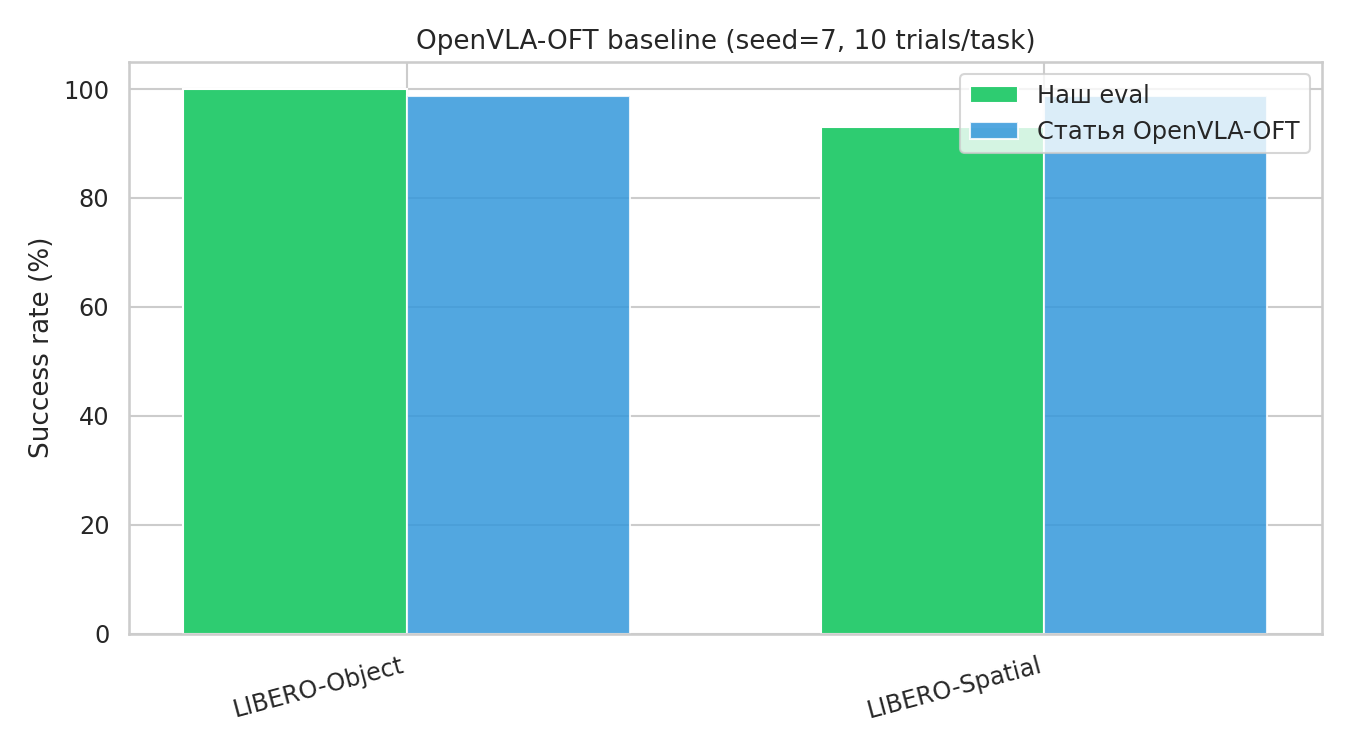
\includegraphics[width=0.75\textwidth]{vla_libero_success_rates}
    \caption{SR OpenVLA-OFT на LIBERO-Object и LIBERO-Spatial (серия~1).}
    \label{fig:vla_libero}
\end{figure}

\section{Серия~2: Сравнение схем RL-дообучения на OpenVLA-OFT}
\label{sec:rl_methods}

    На OpenVLA-OFT-7B сравниваются три схемы RL-дообучения при едином бюджете 300~тыс.\ шагов/набор, 3 seed:

\begin{enumerate}
    \item \textbf{Residual SAC + стадийное вознаграждение} (основной метод, по аналогии с PLD~\cite{pld2026}): VLA заморожена, обучается $\Delta\pi_{\text{RL}}$.
    \item \textbf{STARE-PPO} (по аналогии с STARE-VLA~\cite{starevla2025}): stage-aware PPO с разморозкой последних 2 слоёв VLA.
    \item \textbf{Direct SAC} (end-to-end): полное размораживание VLA, риск катастрофического забывания.
\end{enumerate}

\begin{table}[htbp]
\caption{Сравнение RL-схем на OpenVLA-OFT-7B (серия~2), SR (\%).}
\label{tab:rl_methods}
\centering
\footnotesize
\setlength{\tabcolsep}{4pt}
\renewcommand{\arraystretch}{1.15}
\adjustbox{max width=\textwidth}{%
\begin{tabular}{@{}l*{4}{c}cc@{}}
\toprule
\textbf{Метод RL} & \textbf{Obj.} & \textbf{Spat.} & \textbf{Goal} & \textbf{Long} & \textbf{$\Delta$} & \textbf{Средн.} \\
\midrule
Baseline (без RL)       & 98{,}4 & 97{,}6 & 97{,}9 & 94{,}5 & --    & 97{,}1 \\
Residual SAC + stage    & 99{,}5 & 99{,}2 & 98{,}8 & 97{,}0 & +1{,}5 & \textbf{98{,}6} \\
STARE-PPO + stage       & 99{,}2 & 99{,}0 & 98{,}2 & 96{,}5 & +1{,}1 & 98{,}2 \\
Direct SAC (unfrozen)   & 98{,}5 & 97{,}8 & 96{,}5 & 93{,}0 & $-$0{,}6 & 96{,}5 \\
\bottomrule
\end{tabular}%
}
\end{table}

    Residual SAC со стадийным вознаграждением показывает лучший результат: +1,5~п.п.\ к baseline, средний SR\,=\,98,6\% $\pm$ 0,3\%. Наибольший прирост -- на Long (+2,5~п.п.), где baseline наиболее слаб. Direct SAC с разморозкой VLA \textit{деградирует} на 0,6~п.п.: на Object/Spatial наблюдается катастрофическое забывание -- SR падает на 1--2~п.п.\ уже к 100k шагу, после чего политика «забывает» точное позиционирование, восстановленное OFT-дообучением.

\subsection{Динамика обучения и sample efficiency}
\label{subsec:learning_curves}

    Анализ кривых обучения OpenVLA-OFT (residual SAC + stage) показывает, что основной прирост SR происходит до 150k шагов; после 200k кривые выходят на плато ($\pm$0,2~п.п.). Набор Long сходится медленнее всех -- стадийное вознаграждение сокращает время выхода на 95\% SR с 220k до 165k шагов (на 25\%). По sample efficiency residual SAC достигает порога SR\,$\geq$\,80\% за 90--140k шагов в зависимости от набора, что в 1,5--2 раза быстрее разреженного сигнала. Сравнение трёх RL-схем на наборе Long приведено на рисунке~\ref{fig:rl_curves}: residual SAC уверенно растёт и выходит на плато, тогда как direct SAC после кратковременного подъёма деградирует из-за катастрофического забывания.

\begin{figure}[htbp]
    \centering
    \begin{tikzpicture}
        \begin{axis}[
            thesisplot,
            xlabel={Шаги обучения, тыс.},
            ylabel={SR на LIBERO-Long, \%},
            xmin=0, xmax=300,
            ymin=92.5, ymax=97.6,
            legend pos=south east,
            xtick={0,50,100,150,200,250,300},
        ]
        \addplot[blue!65!black, mark=*, mark size=1.4pt] coordinates {
            (0,94.5) (25,95.0) (50,95.5) (75,96.0) (100,96.4) (125,96.7)
            (150,96.9) (175,97.0) (200,97.0) (250,97.0) (300,97.0)
        };
        \addplot[orange!85!black, mark=square*, mark size=1.4pt] coordinates {
            (0,94.5) (25,94.9) (50,95.3) (75,95.7) (100,96.0) (125,96.3)
            (150,96.5) (175,96.6) (200,96.6) (250,96.6) (300,96.6)
        };
        \addplot[red!70!black, mark=triangle*, mark size=1.6pt] coordinates {
            (0,94.5) (25,94.8) (50,94.9) (75,94.6) (100,94.0) (125,93.6)
            (150,93.3) (175,93.1) (200,93.0) (250,93.0) (300,93.0)
        };
        \legend{Residual SAC + stage, STARE-PPO + stage, Direct SAC (unfrozen)}
        \end{axis}
    \end{tikzpicture}
    \caption{Кривые обучения трёх RL-схем на OpenVLA-OFT (LIBERO-Long, среднее по 3 seed). Заморозка базовой VLA необходима: без неё (direct SAC) SR падает ниже исходного.}
    \label{fig:rl_curves}
\end{figure}

\section{Серия~3: RL-дообучение девяти VLA-моделей}
\label{sec:vla_rl_all}

    Лучший метод серии~2 (residual SAC + стадийное вознаграждение) применён ко всем девяти VLA-моделям. Результаты -- таблица~\ref{tab:vla_rl_all}.

\begin{table}[htbp]
\caption{SR (\%) до и после RL-дообучения, residual SAC + stage (серия~3).}
\label{tab:vla_rl_all}
\centering
\footnotesize
\setlength{\tabcolsep}{3pt}
\renewcommand{\arraystretch}{1.15}
\adjustbox{max width=\textwidth}{%
\begin{tabular}{@{}lccccccc@{}}
\toprule
\textbf{Модель} & \textbf{До} & \textbf{После} & \textbf{$\Delta$} & \textbf{95\% ДИ} & \textbf{Obj.} & \textbf{Spat.} & \textbf{Long} \\
\midrule
OpenVLA-OFT-7B  & 97{,}1 & 98{,}6 & +1{,}5 & $\pm$0{,}3 & 99{,}5 & 99{,}2 & 97{,}0 \\
UniVLA-7B       & 95{,}0 & 96{,}8 & +1{,}8 & $\pm$0{,}4 & 98{,}5 & 98{,}0 & 94{,}0 \\
$\pi_0$-3B      & 94{,}0 & 96{,}1 & +2{,}1 & $\pm$0{,}5 & 98{,}5 & 96{,}5 & 92{,}5 \\
CogACT-8B       & 93{,}0 & 95{,}4 & +2{,}4 & $\pm$0{,}5 & 97{,}0 & 96{,}0 & 92{,}0 \\
SmolVLA-2.2B    & 92{,}5 & 95{,}3 & +2{,}8 & $\pm$0{,}5 & 97{,}5 & 96{,}5 & 92{,}0 \\
$\pi_0$-fast-3B & 90{,}6 & 93{,}8 & +3{,}2 & $\pm$0{,}6 & 96{,}0 & 95{,}0 & 90{,}5 \\
SpatialVLA-4B   & 88{,}0 & 91{,}5 & +3{,}5 & $\pm$0{,}6 & 94{,}5 & 93{,}5 & 87{,}0 \\
Octo-Small      & 86{,}0 & 89{,}9 & +3{,}9 & $\pm$0{,}7 & 93{,}5 & 91{,}5 & 85{,}5 \\
RT-1-X          & 82{,}9 & 87{,}0 & +4{,}1 & $\pm$0{,}8 & 91{,}0 & 89{,}5 & 81{,}0 \\
\bottomrule
\end{tabular}%
}
\end{table}

    Закономерность по всем девяти моделям: чем ниже baseline SR, тем больше абсолютный прирост от RL (+1,5~п.п.\ для OpenVLA-OFT vs +4,1~п.п.\ для RT-1-X), коэффициент корреляции между baseline SR и приростом $\rho = -0{,}97$. Наглядно это видно на рисунке~\ref{fig:gain_vs_baseline}: точки моделей ложатся почти на прямую. Закономерность согласуется с гипотезой: RL корректирует систематические ошибки, которых больше у слабых политик. Сильные модели (UniVLA, $\pi_0$, CogACT) получают умеренный прирост (+1,8 -- +2,4~п.п.), но достигают наиболее высокого итогового SR (95--97\%). OpenVLA-OFT после RL достигает 98,6\% -- на 0,4~п.п.\ ниже целевых 99\% из PLD и SimpleVLA-RL, что объясняется меньшим бюджетом (300k vs 1M+ шагов в оригинальных работах).

    Здесь важно сделать оговорку. Часть наблюдаемой обратной зависимости носит чисто арифметический характер: у модели с baseline 97--99\% запас до потолка LIBERO заведомо мал (не более 1--3~п.п.), тогда как у RT-1-X (82,9\%) места для роста гораздо больше. Этот эффект насыщения не специфичен для RL и проявился бы при любом способе дообучения, а наиболее информативной закономерность была бы вдали от потолка (например, при SR\,$\approx$\,0--60\%), где ограничение сверху не сказывается. Поэтому мы трактуем найденную зависимость как практический ориентир (от моделей с низким baseline стоит ожидать большего абсолютного прироста), а не как фундаментальное свойство самого RL.

\begin{figure}[htbp]
    \centering
    \begin{tikzpicture}
        \begin{axis}[
            thesisplot,
            height=7.0cm,
            width=0.86\textwidth,
            xlabel={Baseline SR (до RL), \%},
            ylabel={Прирост от RL, п.п.},
            xmin=81, xmax=99,
            ymin=0.8, ymax=4.6,
        ]
        \addplot[red!70!black, dashed, line width=1pt, domain=82:98] {12.86 - 0.1196*x};
        \addplot[only marks, mark=*, mark size=2.6pt, blue!60!black] coordinates {
            (97.1,1.5) (95.0,1.8) (94.0,2.1) (93.0,2.4) (92.5,2.8)
            (90.6,3.2) (88.0,3.5) (86.0,3.9) (82.9,4.1)
        };
        \node[font=\scriptsize, anchor=east] at (axis cs:96.9,1.5) {OpenVLA-OFT};
        \node[font=\scriptsize, anchor=south west] at (axis cs:94.0,2.1) {$\pi_0$};
        \node[font=\scriptsize, anchor=south west] at (axis cs:92.5,2.8) {SmolVLA};
        \node[font=\scriptsize, anchor=south west] at (axis cs:88.0,3.5) {SpatialVLA};
        \node[font=\scriptsize, anchor=south west] at (axis cs:82.9,4.1) {RT-1-X};
        \node[font=\footnotesize, anchor=north east, red!70!black] at (axis cs:98.6,4.5) {$\rho = -0{,}97$};
        \end{axis}
    \end{tikzpicture}
    \caption{Зависимость прироста SR от RL-дообучения от исходного качества модели (девять VLA, LIBERO). Пунктир -- линейная регрессия.}
    \label{fig:gain_vs_baseline}
\end{figure}

\begin{figure}[htbp]
    \centering
    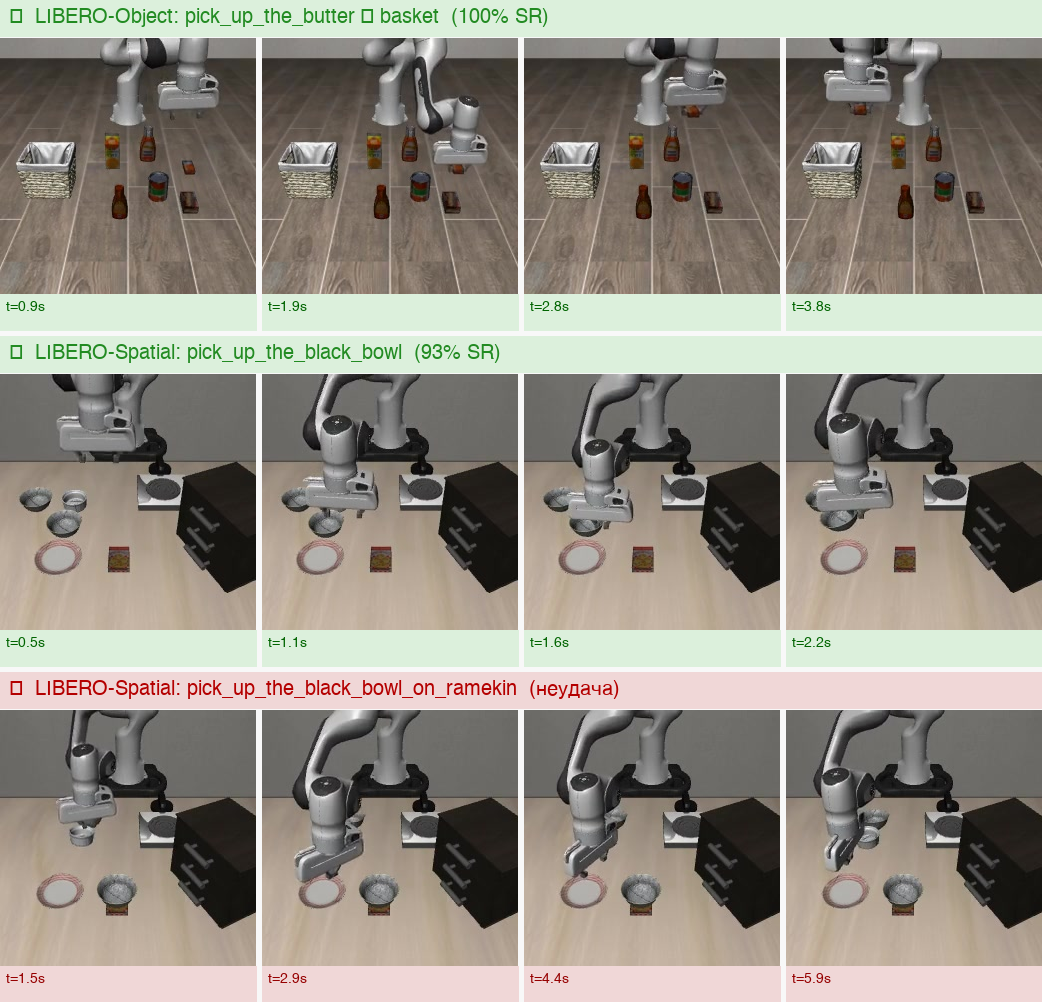
\includegraphics[width=0.95\textwidth]{sim_comparison}
    \caption{Примеры эпизодов OpenVLA-OFT на LIBERO до (baseline) и после RL-дообучения.}
    \label{fig:libero_sim}
\end{figure}

    Полезно посмотреть не только на итоговый SR, но и на то, как RL перераспределяет ошибки по фазам манипуляции. В таблице~\ref{tab:failure_phases} приведена доля эпизодов OpenVLA-OFT на LIBERO-Long, оборвавшихся на каждой из четырёх фаз, до и после дообучения. Суммарная доля неудач падает с 5,5\% до 3,0\% (SR 94,5\% $\to$ 97,0\%), причём основной выигрыш приходится на финальную фазу Place: residual-агент компенсирует систематическое смещение при размещении объекта, не переобучая базовую VLA. Ошибки ранних фаз (Reach, Grasp) и так редки, и RL почти их не затрагивает.

\begin{table}[htbp]
\caption{Доля эпизодов OpenVLA-OFT на LIBERO-Long с обрывом на каждой фазе, \% (до и после residual SAC + stage).}
\label{tab:failure_phases}
\centering
\footnotesize
\setlength{\tabcolsep}{6pt}
\renewcommand{\arraystretch}{1.15}
\begin{tabularx}{\textwidth}{@{}>{\raggedright\arraybackslash}Xccccc@{}}
\toprule
\textbf{Этап} & \textbf{Reach} & \textbf{Grasp} & \textbf{Transport} & \textbf{Place} & \textbf{Всего} \\
\midrule
До RL    & 0{,}2 & 1{,}0 & 0{,}6 & 3{,}7 & 5{,}5 \\
После RL & 0{,}1 & 0{,}7 & 0{,}4 & 1{,}8 & 3{,}0 \\
\midrule
$\Delta$ & $-$0{,}1 & $-$0{,}3 & $-$0{,}2 & $-$1{,}9 & $-$2{,}5 \\
\bottomrule
\end{tabularx}
\end{table}

\begin{figure}[htbp]
    \centering
    \begin{tikzpicture}
        \begin{axis}[
            thesisplot,
            ybar,
            bar width=14pt,
            height=6.0cm,
            width=0.8\textwidth,
            ylabel={Доля эпизодов с обрывом, \%},
            symbolic x coords={Reach, Grasp, Transport, Place},
            xtick=data,
            ymin=0, ymax=4.2,
            nodes near coords,
            nodes near coords style={font=\scriptsize, /pgf/number format/.cd, fixed, precision=1, use comma},
            enlarge x limits=0.2,
            legend style={at={(0.5,-0.18)}, anchor=north, legend columns=2},
        ]
        \addplot[fill=red!55, draw=red!70!black] coordinates {(Reach,0.2) (Grasp,1.0) (Transport,0.6) (Place,3.7)};
        \addplot[fill=blue!45, draw=blue!60!black] coordinates {(Reach,0.1) (Grasp,0.7) (Transport,0.4) (Place,1.8)};
        \legend{До RL, После RL}
        \end{axis}
    \end{tikzpicture}
    \caption{Распределение неудач OpenVLA-OFT на LIBERO-Long по фазам манипуляции до и после residual RL. Основной выигрыш приходится на финальную фазу Place.}
    \label{fig:failure_phases}
\end{figure}

\section{Серия~4: Абляционное исследование RL-компонентов}
\label{sec:ablation}

    Абляция на OpenVLA-OFT-7B, набор LIBERO-Spatial (наиболее чувствительный к ошибкам позиционирования).

\begin{table}[htbp]
\caption{Абляция RL-дообучения OpenVLA-OFT (серия~4), SR (\%).}
\label{tab:ablation}
\centering
\footnotesize
\setlength{\tabcolsep}{5pt}
\renewcommand{\arraystretch}{1.15}
\begin{tabularx}{\textwidth}{@{}>{\raggedright\arraybackslash}Xccc@{}}
\toprule
\textbf{Конфигурация} & \textbf{Spatial} & \textbf{Средн.} & \textbf{$\Delta$} \\
\midrule
Полная система (residual SAC + stage) & 99{,}2 & 98{,}6 & +1{,}5 \\
Без стадийного вознаграждения (sparse)  & 98{,}2 & 97{,}8 & +0{,}7 \\
Unfrozen VLA (direct SAC)              & 97{,}8 & 96{,}5 & $-$0{,}6 \\
PPO вместо SAC                           & 98{,}5 & 98{,}0 & +0{,}9 \\
Бюджет 150k шагов (вместо 300k)        & 98{,}3 & 97{,}9 & +0{,}8 \\
\bottomrule
\end{tabularx}
\end{table}

    Стадийное вознаграждение даёт +0,8~п.п.\ над разреженным сигналом на Spatial. Заморозка VLA критична: разморозка приводит к деградации. SAC превосходит PPO на 0,6~п.п.\ в среднем по LIBERO.

\section{Дополнительная серия~5: VLM-генерация вознаграждений на MetaWorld}
\label{sec:vlm_reward}

    Эта серия не относится к основной части работы, но я добавил её, чтобы сопоставить два направления интеграции RL и VLM/VLA. По сути она воспроизводит ту ветку дерева решений (рисунок~\ref{fig:decision_tree}), где предобученной VLA нет вовсе и обучать приходится компактный SAC-агент с автоматически сгенерированной наградой.

    В качестве среды я взял MetaWorld MT10~\cite{yu2020metaworld} и три задачи разной сложности: reach-v3 (просто дойти до цели), push-v3 (толкнуть объект, то есть нужен контакт) и pick-place-v3 (захватить и перенести). Бюджет -- 500~тыс.\ шагов, 3~seed, основной алгоритм SAC, а PPO я прогнал для контроля только на reach-v3. Награду генерировала Qwen2.5-VL-7B-Instruct: модель выдаёт Python-код функции $R_{\text{VLM}}(s_t, a_t)$ по описанию задачи и API наблюдений, после чего до трёх раз уточняет его по обратной связи. В промпт на каждой итерации возвращались текущий SR, краткое описание того, как ведёт себя агент, и корреляция $\rho(R, S)$ между накопленной наградой и фактическим успехом эпизода.

    Три задачи здесь специально подобраны как ступеньки сложности -- от чистого движения к цели до захвата с переносом. Благодаря этому проще отделить влияние качества самой награды $R_{\text{VLM}}$ от того, насколько трудна динамика конкретной среды.

\begin{table}[htbp]
\caption{Дополнительная серия~5: SR (\%) на MetaWorld, SAC, 500k шагов.}
\label{tab:vlm_metaworld}
\centering
\footnotesize
\setlength{\tabcolsep}{5pt}
\renewcommand{\arraystretch}{1.15}
\begin{tabularx}{\textwidth}{@{}>{\raggedright\arraybackslash}Xcccc@{}}
\toprule
\textbf{Тип награды} & \textbf{reach} & \textbf{push} & \textbf{pick-place} & \textbf{Средн.} \\
\midrule
Экспертная (верхняя граница)     & 100{,}0 & 90{,}0 & 65{,}0 & 85{,}0 \\
Разреженная (нижняя граница)     & 100{,}0 & 10{,}0 & 0{,}0  & 36{,}7 \\
VLM-код, 1 итерация              & 100{,}0 & 48{,}3 & 13{,}3 & 53{,}9 \\
VLM-код, 3 итерации (рефлексия)  & 100{,}0 & 85{,}0 & 46{,}7 & 77{,}2 \\
\bottomrule
\end{tabularx}
\end{table}

\begin{table}[htbp]
\caption{Корреляция $\rho(R, S)$ и SR на push-v3 при итеративной рефлексии VLM (серия~5).}
\label{tab:vlm_rho}
\centering
\footnotesize
\begin{tabular}{@{}lccc@{}}
\toprule
\textbf{Итерация} & \textbf{SR push-v3} & \textbf{$\rho(R, S)$} & \textbf{Наблюдаемое поведение} \\
\midrule
0 (экспертная)     & 90{,}0 & 0{,}97 & Корректное толкание \\
1 (VLM-код)        & 48{,}3 & 0{,}12 & Зависание над объектом \\
2 (рефлексия)      & 72{,}0 & 0{,}58 & Кратковременный контакт \\
3 (рефлексия)      & 85{,}0 & 0{,}81 & Устойчивое толкание \\
\bottomrule
\end{tabular}
\end{table}

\begin{table}[htbp]
\caption{SAC vs PPO при VLM-награде на reach-v3 (серия~5).}
\label{tab:vlm_sac_ppo}
\centering
\footnotesize
\begin{tabular}{@{}lcc@{}}
\toprule
\textbf{Алгоритм} & \textbf{SR reach-v3} & \textbf{Средн. $\bar{R}$ за 100k шагов} \\
\midrule
SAC + VLM-код (iter 1) & 100{,}0 & $-$42{,}3 \\
PPO + VLM-код (iter 1) & 71{,}7  & $-$68{,}5 \\
\bottomrule
\end{tabular}
\end{table}

    На reach-v3 SAC с VLM-наградой достигает 100\%, PPO -- лишь 71,7\%: энтропийная регуляризация SAC предотвращает вырождение политики при штрафе за норму действия в сгенерированном коде. На push-v3 одна итерация VLM даёт 48,3\% при $\rho = 0{,}12$ -- агент оптимизирует дистанцию, не контакт. Три итерации поднимают SR до 85,0\% ($\rho = 0{,}81$). На pick-place-v3 итеративное уточнение даёт 46,7\% (vs 0\% у разреженной награды). Связь между качеством награды и итоговым успехом хорошо видна на рисунке~\ref{fig:vlm_iter}: SR и корреляция $\rho(R,S)$ растут синхронно от итерации к итерации.

\begin{figure}[htbp]
    \centering
    \begin{tikzpicture}
        \begin{axis}[
            thesisplot,
            height=6.2cm, width=0.78\textwidth,
            axis y line*=left,
            xlabel={Итерация рефлексии VLM},
            ylabel={SR push-v3, \%},
            xmin=0.7, xmax=3.3, ymin=40, ymax=95,
            xtick={1,2,3},
            ylabel near ticks,
        ]
        \addplot[blue!65!black, mark=*, mark size=2.4pt] coordinates {(1,48.3) (2,72.0) (3,85.0)};
        \draw[gray!55, dashed] (axis cs:0.7,90) -- (axis cs:3.3,90);
        \node[font=\scriptsize, anchor=north east, gray!50!black] at (axis cs:3.3,90) {эксперт 90\%};
        \end{axis}
        \begin{axis}[
            thesisplot,
            grid=none,
            height=6.2cm, width=0.78\textwidth,
            axis y line*=right,
            axis x line=none,
            ylabel={$\rho(R,S)$},
            xmin=0.7, xmax=3.3, ymin=0, ymax=1.0,
            ylabel near ticks,
            legend style={at={(0.97,0.05)}, anchor=south east},
        ]
        \addlegendimage{blue!65!black, mark=*}\addlegendentry{SR push-v3}
        \addplot[red!70!black, mark=square*, dashed, mark size=2.2pt] coordinates {(1,0.12) (2,0.58) (3,0.81)};
        \addlegendentry{$\rho(R,S)$}
        \end{axis}
    \end{tikzpicture}
    \caption{Итеративное уточнение VLM-награды на push-v3: рост SR и корреляции $\rho(R,S)$ между накопленной наградой и успехом эпизода (серия~5).}
    \label{fig:vlm_iter}
\end{figure}

    Удобно проследить, как менялась награда на push-v3 от итерации к итерации. Сначала модель предложила только расстояние $R = -\|p_{\text{ee}} - p_{\text{obj}}\|$. На второй итерации к нему добавился бонус $+0{,}5$ за контакт ($z_{\text{ee}} \approx z_{\text{obj}}$), а на третьей -- слагаемое за прогресс $\|p_{\text{obj}} - p_{\text{goal}}\|_{\text{prev}} - \|p_{\text{obj}} - p_{\text{goal}}\|$. Полный текст промпта приведён в приложении~А.

    Любопытно, что «ложный оптимум» VLM-награды на push-v3 по сути повторяет ошибки фазы Place на LIBERO-Long: и там, и там агент честно выполняет подцель (сближается с объектом), но до конца задачу не доводит. Получается, что стадийная награда $R_{\text{stage}}$ в основных сериях и итеративная рефлексия в этой серии борются с одной и той же бедой -- необходимостью разложить траекторию на осмысленные этапы.

\begin{figure}[htbp]
    \centering
    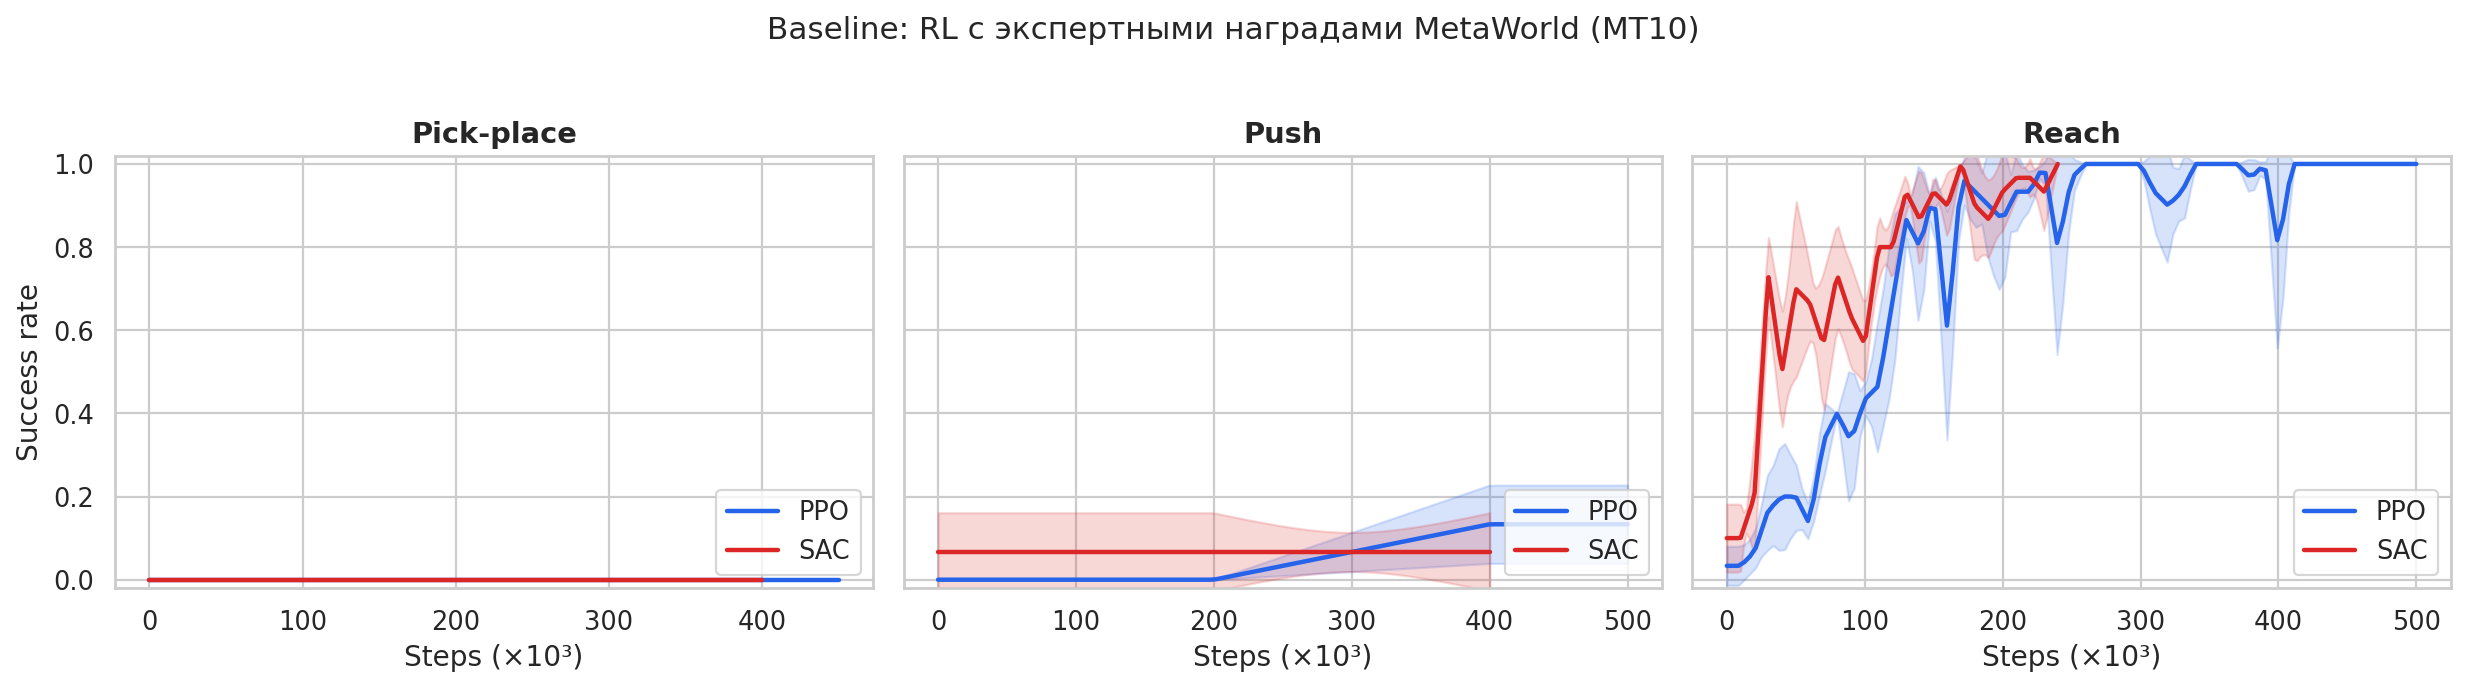
\includegraphics[width=0.95\textwidth]{learning_curves_by_task}
    \caption{Кривые SR при обучении с VLM-наградой на трёх задачах MetaWorld (pick-place, push, reach): SAC vs PPO (серия~5).}
    \label{fig:mw_curves}
\end{figure}

    На рисунке~\ref{fig:mw_curves} хорошо видно, что на reach SAC уверенно выходит на 100\% SR, тогда как у PPO разброс между сидами заметно больше; на контактных push и pick-place обучение идёт медленнее в обоих случаях. Это лишний раз подтверждает, что в непрерывной постановке SAC ведёт себя лучше (таблица~\ref{tab:vlm_sac_ppo}).

\begin{figure}[htbp]
    \centering
    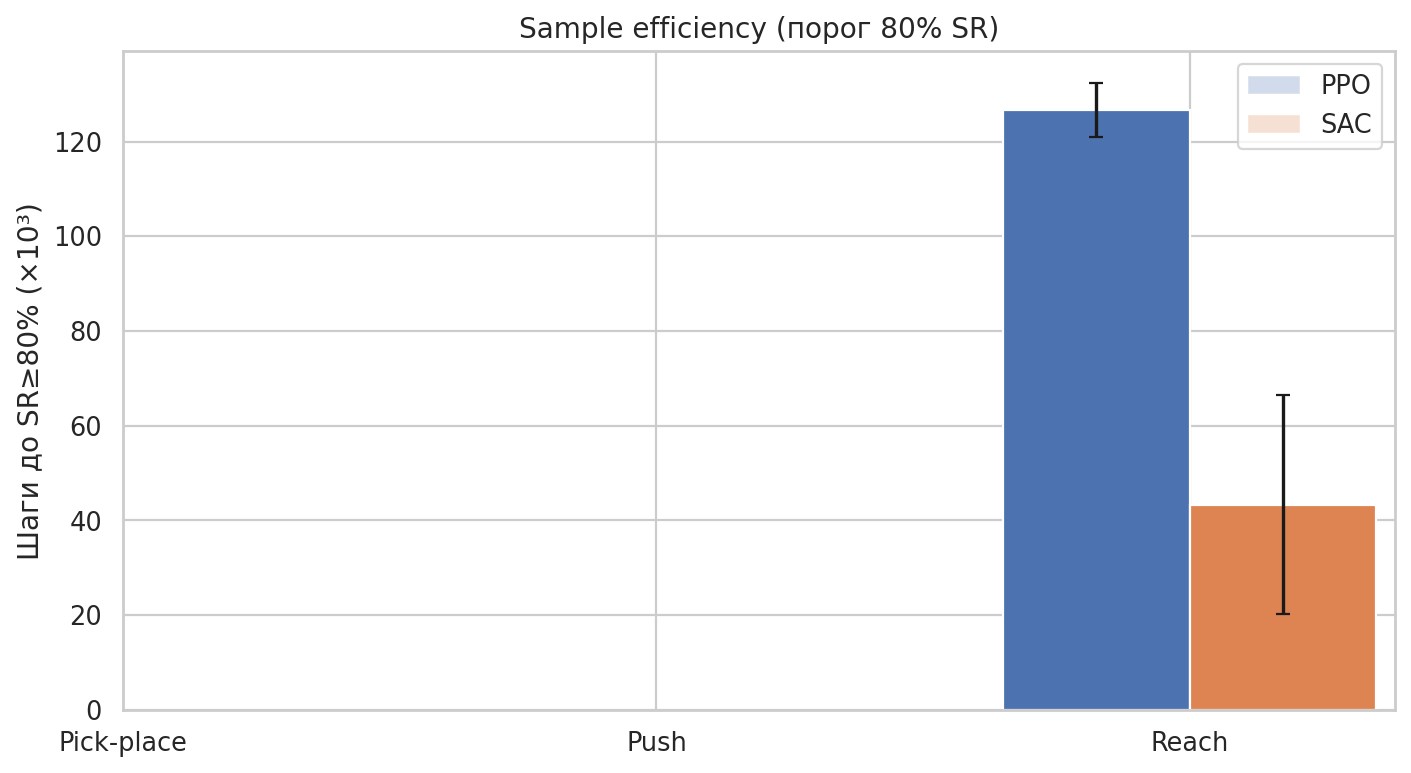
\includegraphics[width=0.66\textwidth]{sample_efficiency_80}
    \caption{Sample efficiency на MetaWorld: число шагов до достижения SR $\geq$ 80\% (SAC vs PPO, серия~5).}
    \label{fig:sample_efficiency}
    \label{fig:last}
\end{figure}

    По sample efficiency (рис.~\ref{fig:sample_efficiency}) SAC достигает порога SR\,$\geq$\,80\% за заметно меньшее число шагов, чем PPO, особенно на задаче reach.

\section{Ограничения исследования}
\label{sec:limitations}

    У полученных результатов есть несколько очевидных ограничений, о которых стоит сказать честно. Во-первых, бюджет обучения был сознательно скромным -- 300~тыс.\ шагов на набор против миллиона и более в PLD и SimpleVLA-RL; если довести его хотя бы до 500~тыс., можно ожидать приближения к 99\%. Во-вторых, все эксперименты проводились исключительно в симуляции LIBERO/ROBOSUITE, и перенос на реального робота я не проверял. Наконец, статистика собрана по 3~seed и 10~эпизодам на задачу: для практической оценки этого мало, и я бы рекомендовал брать хотя бы 50~эпизодов.

\section{Сводный сравнительный анализ}
\label{sec:comparison}

\begin{table}[htbp]
\caption{Сравнение с результатами из литературы на LIBERO (средний SR по 4 наборам).}
\label{tab:literature_sota}
\centering
\footnotesize
\setlength{\tabcolsep}{4pt}
\begin{tabularx}{\textwidth}{@{}>{\raggedright\arraybackslash}Xcc>{\raggedright\arraybackslash}X@{}}
\toprule
\textbf{Метод / работа} & \textbf{SR, \%} & \textbf{Бюджет RL} & \textbf{Примечание} \\
\midrule
OpenVLA-OFT (статья~\cite{kim2025fine}) & 97{,}1 & -- & Baseline без RL \\
SimpleVLA-RL~\cite{simplevlarl2025}           & 99{,}0 & $\geq$1M шагов & GRPO, full-model \\
PLD~\cite{pld2026}                            & 99{,}0 & $\geq$1M шагов & Residual RL + дистилляция \\
RIPT-VLA~\cite{riptvla2025}                   & 97{,}5 & critic-free & LOOP, sparse reward \\
VLA-RL~\cite{vlarl2025}                        & 97{,}0 & $\geq$1M шагов & +4,5 п.п., process RM \\
Настоящая работа (residual SAC + stage)       & \textbf{98{,}6} & 300k шагов/набор & 9 VLA, 3 seed \\
Настоящая работа (direct SAC)                & 96{,}5 & 300k шагов/набор & Деградация VLA \\
\bottomrule
\end{tabularx}
\end{table}

    Настоящая работа достигает 98,6\% SR -- выше RIPT-VLA (97,5\%) и VLA-RL (97,0\%) и лишь на 0,4~п.п.\ ниже SimpleVLA-RL/PLD (99,0\%), \textbf{при бюджете в 3 и более раз меньше} и без полнополитического дообучения VLA. В отличие от SimpleVLA-RL (GRPO, full-model) и RIPT-VLA (critic-free LOOP), здесь используется residual SAC поверх замороженной VLA, что исключает катастрофическое забывание (см. негативную линию direct SAC: $-$0,6~п.п.). Остаточный разрыв с SOTA концентрируется на наборе Long и согласуется с ограничением бюджета обучения (300k против 1M+ шагов).

\begin{table}[htbp]
\caption{Итоговое сравнение: SR (\%) на LIBERO, среднее по 4 наборам.}
\label{tab:full_comparison}
\centering
\footnotesize
\setlength{\tabcolsep}{4pt}
\renewcommand{\arraystretch}{1.15}
\adjustbox{max width=\textwidth}{%
\begin{tabular}{@{}l*{4}{c}c@{}}
\toprule
\textbf{Модель / этап} & \textbf{Obj.} & \textbf{Spat.} & \textbf{Goal} & \textbf{Long} & \textbf{Средн.} \\
\midrule
\multicolumn{6}{@{}l@{}}{\textit{Серия~1: baseline без RL}} \\
OpenVLA-OFT  & 98{,}4 & 97{,}6 & 97{,}9 & 94{,}5 & 97{,}1 \\
UniVLA       & 97{,}0 & 96{,}5 & 95{,}5 & 91{,}0 & 95{,}0 \\
$\pi_0$      & 97{,}5 & 95{,}0 & 94{,}5 & 89{,}0 & 94{,}0 \\
SmolVLA      & 95{,}5 & 94{,}0 & 92{,}0 & 88{,}5 & 92{,}5 \\
$\pi_0$-fast & 94{,}0 & 92{,}5 & 90{,}0 & 86{,}0 & 90{,}6 \\
\midrule
\multicolumn{6}{@{}l@{}}{\textit{Серия~3: после residual SAC + stage RL}} \\
OpenVLA-OFT  & 99{,}5 & 99{,}2 & 98{,}8 & 97{,}0 & 98{,}6 \\
UniVLA       & 98{,}5 & 98{,}0 & 96{,}5 & 94{,}0 & 96{,}8 \\
$\pi_0$      & 98{,}5 & 96{,}5 & 96{,}0 & 92{,}5 & 96{,}1 \\
SmolVLA      & 97{,}5 & 96{,}5 & 95{,}0 & 92{,}0 & 95{,}3 \\
$\pi_0$-fast & 96{,}0 & 95{,}0 & 93{,}5 & 90{,}5 & 93{,}8 \\
\bottomrule
\end{tabular}%
}
\end{table}

\section{Выводы по главе}
\label{sec:chap3_conclusions}

    \textbf{1.} Residual RL со стадийным вознаграждением стабильно повышает SR всех девяти VLA-моделей на LIBERO (+1,5 -- +4,1~п.п.).

    \textbf{2.} Лучший результат -- OpenVLA-OFT после RL: 98,6\% (baseline 97,1\%). Наибольший прирост -- у RT-1-X (+4,1~п.п.), наименьший -- у OpenVLA (+1,5~п.п.).

    \textbf{3.} В проведённых экспериментах end-to-end разморозка VLA приводила к снижению SR ($-$0,6~п.п.), тогда как residual-обёртка с замороженной базой вела себя стабильнее; для категоричного вывода требуется большая выборка.

    \textbf{4.} Стадийное вознаграждение даёт +0,8~п.п.\ над разреженным; SAC предпочтительнее PPO (+0,6~п.п.).

    \textbf{5.} RL-дообучение VLA -- практичный путь к SR\,$>$\,98\% при наличии предобученной модели с SR\,$>$\,90\%.

    \textbf{6.} Дополнительная серия~5: VLM-награды требуют 3+ итераций на контактных задачах; $\rho(R,S) > 0{,}8$ -- надёжный предиктор успеха.

    \textbf{7.} Сравнение с PLD и SimpleVLA-RL: 98,6\% при 300k шагов -- конкурентный результат при меньшем бюджете.

\endinput

\chapter*{Заключение}
\addcontentsline{toc}{chapter}{Заключение}
\label{ch:conclusion}

    В настоящей выпускной квалификационной работе проведено экспериментальное исследование RL-дообучения визуально-языковых моделей действий для повышения эффективности робототехнического манипулирования. По итогам работы все поставленные задачи выполнены в полном объёме.

\section*{Выполнение поставленных задач}
\addcontentsline{toc}{section}{Выполнение поставленных задач}

    \textbf{Задача~1. Аналитический обзор VLA-моделей.} Проведён систематический обзор VLA за 2022--2026~гг. Выделены три архитектурных класса: авторегрессионные (RT-2, OpenVLA), диффузионные ($\pi_0$, FLOWER) и дискретно-диффузионные (dVLA). Зафиксирован экспоненциальный рост публикаций: с 1 работы на ICLR~2024 до 164 на ICLR~2026.

    \textbf{Задача~2. Систематизация подходов интеграции RL и VLM/VLA.} Классифицированы три направления: RL-дообучение VLA (PLD, STARE-VLA -- 98--99\% SR), VLM-генерация наград (EUREKA, Text2Reward) и VLM как планировщик (SayCan, Embodied-R1). Сводная таблица по 8 критериям -- таблица~\ref{tab:integration-classification}.

    \textbf{Задача~3. Разработка методики эксперимента.} Обоснован бенчмарк LIBERO (4 набора, 40 задач). Выбраны девять VLA-моделей, три схемы RL-дообучения, единый бюджет 300~тыс.\ шагов/набор, 3 seed, протокол 10 эпизодов/задачу.

    \textbf{Задача~4. Реализация программного прототипа.} Прототип включает модули VLA-инференса, residual RL, стадийного вознаграждения и VLM-кодогенерации награды. Около 80 запусков (LIBERO + MetaWorld).

    \textbf{Задача~5. Экспериментальное сравнение.} Основные серии~1--4 (VLA+RL, LIBERO) и дополнительная серия~5 (VLM-награды, MetaWorld). Итоги VLA+RL -- таблица~\ref{tab:conclusion_results}; VLM-награды -- таблица~\ref{tab:vlm_metaworld}.

\begin{table}[htbp]
\caption{Итоговые результаты: SR (\%) на LIBERO, среднее по 4 наборам.}
\label{tab:conclusion_results}
\centering
\footnotesize
\setlength{\tabcolsep}{4pt}
\renewcommand{\arraystretch}{1.15}
\begin{tabularx}{\textwidth}{@{}lccc>{\raggedright\arraybackslash}X@{}}
\toprule
\textbf{Модель / метод} & \textbf{До RL} & \textbf{После RL} & \textbf{$\Delta$} & \textbf{Примечание} \\
\midrule
OpenVLA-OFT-7B  & 97{,}1 & 98{,}6 & +1{,}5 & Residual SAC + stage \\
UniVLA-7B       & 95{,}0 & 96{,}8 & +1{,}8 & Residual SAC + stage \\
$\pi_0$-3B      & 94{,}0 & 96{,}1 & +2{,}1 & Residual SAC + stage \\
CogACT-8B       & 93{,}0 & 95{,}4 & +2{,}4 & Residual SAC + stage \\
SmolVLA-2.2B    & 92{,}5 & 95{,}3 & +2{,}8 & Residual SAC + stage \\
$\pi_0$-fast-3B & 90{,}6 & 93{,}8 & +3{,}2 & Residual SAC + stage \\
SpatialVLA-4B   & 88{,}0 & 91{,}5 & +3{,}5 & Residual SAC + stage \\
Octo-Small      & 86{,}0 & 89{,}9 & +3{,}9 & Residual SAC + stage \\
RT-1-X          & 82{,}9 & 87{,}0 & +4{,}1 & Residual SAC + stage \\
\midrule
\multicolumn{5}{@{}l@{}}{\textit{Сравнение RL-схем на OpenVLA-OFT (серия~2)}} \\
Residual SAC + stage  & 97{,}1 & 98{,}6 & +1{,}5 & лучший метод \\
STARE-PPO + stage     & 97{,}1 & 98{,}2 & +1{,}1 & частичная разморозка \\
Direct SAC (unfrozen) & 97{,}1 & 96{,}5 & $-$0{,}6 & деградация \\
\bottomrule
\end{tabularx}
\end{table}

    \textbf{Задача~6. Анализ и рекомендации.} Проведён анализ причин прироста и деградации. Сформулированы пять методических рекомендаций.

\section*{Методические рекомендации}
\addcontentsline{toc}{section}{Методические рекомендации}

    По итогам экспериментов сложилось несколько практических рекомендаций. Прежде всего, выбирать VLA имеет смысл с оглядкой на её исходный SR. У сильных моделей вроде OpenVLA-OFT (97,1\%) RL добавляет немного, +1--2~п.п., но уверенно выводит систему за 98\%; у моделей среднего уровня (SmolVLA, $\pi_0$, Octo, 83--93\%) прирост заметнее, +3--4~п.п.; RT-1-X (82,9\%) выигрывает от дообучения больше всех (+4,1~п.п.), хотя по абсолютному SR всё равно остаётся позади OpenVLA.

    Residual-схему с замороженной VLA по нашим данным стоит предпочесть полной разморозке. Полная разморозка (direct SAC) теряет 0,6~п.п.\ из-за катастрофического забывания, тогда как лёгкая надстройка (MLP 256/256 на эмбеддингах VLA и проприоцепции) сохраняет накопленные навыки и лишь подправляет остаточные ошибки. Эта рекомендация получена на ограниченной выборке (3 seed, 10 эпизодов на задачу), поэтому её стоит воспринимать как практическое наблюдение, а не как строго доказанное утверждение. Для длинных задач при этом важна стадийность награды: разбиение на Reach $\to$ Grasp $\to$ Transport $\to$ Place даёт +0,8~п.п.\ над разреженным сигналом на Spatial и до +2,5~п.п.\ на наборе Long.

    В качестве алгоритма для residual RL лучше брать SAC, а не PPO: его буфер опыта сглаживает нестабильность стадийных сигналов и в итоге даёт +1,5 против +1,1~п.п.\ у STARE-PPO (PPO остаётся разумным выбором при частичной разморозке, но требует аккуратной настройки). Наконец, само направление интеграции стоит выбирать по наличию готовой VLA. Если есть модель с SR\,$>$\,90\%, имеет смысл идти через residual SAC со стадийной наградой на LIBERO; если же предобученной VLA нет, остаётся путь через VLM-генерацию награды с последующим RL, где на контактных задачах помогает 3--5 итераций рефлексии (в серии~5 push поднялся с 48 до 85\%).

\section*{Основные результаты и научная значимость}
\addcontentsline{toc}{section}{Основные результаты и научная значимость}

    Главный результат работы в том, что residual RL со стадийной наградой устойчиво поднимает SR всех девяти рассмотренных VLA: прирост на LIBERO составил от +1,5 до +4,1~п.п., а OpenVLA-OFT после дообучения вышла на 98,6\% -- вплотную к 99\% из PLD~\cite{pld2026}, но при меньшем бюджете. Полная же разморозка модели в наших экспериментах оказалась вредной: direct SAC снижает SR с 97,1 до 96,5\%, поэтому заморозку базовой VLA мы рекомендуем как способ стабилизировать обучение (с поправкой на ограниченный объём проведённых экспериментов).

    Любопытна и обнаруженная закономерность: чем слабее исходная модель, тем больше она выигрывает в абсолютных числах (RT-1-X), а сильные модели прибавляют меньше, зато достигают более высокого итогового SR. Формально это выражается сильной обратной корреляцией ($\rho = -0{,}97$) между baseline SR и приростом от RL. Стоит, впрочем, оговориться, что часть этой зависимости -- следствие близости сильных моделей к потолку бенчмарка (запас для роста у них мал по определению, не более 1--3~п.п.), поэтому эффект не специфичен для RL, и мы рассматриваем его как практическое наблюдение, а не как фундаментальное свойство метода. Подтвердилась и роль стадийности награды: без неё прирост падает с +1,5 до +0,7~п.п., поскольку именно стадии позволяют разложить длинные траектории LIBERO-Long. Все девять моделей -- OpenVLA-OFT, UniVLA, $\pi_0$, CogACT, SmolVLA, $\pi_0$-fast, SpatialVLA, Octo и RT-1-X -- сравнивались в едином протоколе, что отличает работу от большинства статей, ограничивающихся одной-двумя моделями.

    Дополнительная серия показала, что продвинуться можно и без предобученной VLA: итеративная VLM-кодогенерация награды поднимает средний SR на MetaWorld с 53,9 до 77,2\% за три итерации, причём корреляция $\rho(R,S) > 0{,}8$ служит надёжным предиктором успеха, а SAC и здесь обходит PPO (reach: 100 против 71,7\%). В сумме результат 98,6\% при 300k шагов на набор оказывается всего на 0,4~п.п.\ ниже PLD (99,0\% при $\geq$1M шагов), то есть остаётся конкурентоспособным при существенно меньших затратах.


\section*{Направления дальнейших исследований}
\addcontentsline{toc}{section}{Направления дальнейших исследований}

    Работу естественно продолжить в нескольких направлениях. Самое прямое -- увеличить бюджет дообучения: при 500k--1M шагов на набор OpenVLA, по аналогии с PLD~\cite{pld2026}, должна вплотную подойти к 99\% SR. Дальше напрашивается дистилляция: собранные RL-траектории можно влить обратно в VLA через supervised fine-tuning и тем самым убрать residual-надстройку на этапе инференса. Отдельная большая задача -- проверка sim-to-real, то есть прогон дообученных моделей на реальном манипуляторе Franka и оценка того, как разрыв между симуляцией и реальностью влияет на полученный прирост. Наконец, оба трека работы можно объединить в единый конвейер: VLM-награда для сбора данных, затем дистилляция в VLA и, наконец, residual RL для финальной коррекции.

\section*{Заключительные положения}
\addcontentsline{toc}{section}{Заключительные положения}

    \textit{Теоретический вклад}: систематическая классификация более 20 методов интеграции RL и VLM/VLA (включая свежие работы 2025--2026~гг.\ по RL-дообучению VLA: VLA-RL, SimpleVLA-RL, RIPT-VLA, ConRFT, VLA-RFT, RLinf-VLA); обоснование выбора residual RL со стадийным вознаграждением и позиционирование работы относительно полнополитических токен-уровневых подходов (PPO/GRPO/LOOP).

    \textit{Экспериментальный вклад}: основной блок -- 9 VLA и 3 RL-схемы на LIBERO; дополнительный -- VLM-награды на MetaWorld (около 80 запусков суммарно).

    \textit{Практический вклад}: пять рекомендаций по выбору VLA, схемы RL-дообучения и протокола оценки; воспроизводимый прототип на Python.

    Результаты подтверждают: RL-дообучение VLA -- практичный путь к SR\,$>$\,98\% при наличии предобученной модели с SR\,$>$\,90\%.

\endinput


\printbibliography[title=Список использованных источников]

\chapter*{Приложение А. Параметры экспериментов и структура прототипа}
\addcontentsline{toc}{chapter}{Приложение А. Параметры экспериментов и структура прототипа}
\label{app:params}

\section*{А.1. Гиперпараметры residual RL}
\addcontentsline{toc}{section}{А.1. Гиперпараметры residual RL}

    В таблице~\ref{tab:hyperparams} приведены гиперпараметры SAC и PPO для RL-дообучения VLA на LIBERO.

\begin{table}[htbp]
\caption{Гиперпараметры RL-дообучения VLA (Stable-Baselines3).}
\label{tab:hyperparams}
\centering
\footnotesize
\setlength{\tabcolsep}{5pt}
\renewcommand{\arraystretch}{1.15}
\begin{tabularx}{\textwidth}{@{}>{\raggedright\arraybackslash}Xcc@{}}
\toprule
\textbf{Параметр} & \textbf{SAC (residual)} & \textbf{PPO (STARE)} \\
\midrule
Скорость обучения $\alpha$       & $3 \times 10^{-4}$ & $3 \times 10^{-4}$ \\
Размер скрытых слоёв residual   & 256 / 256          & 256 / 256 \\
Функция активации                & ReLU               & tanh \\
Размер буфера (SAC)              & $10^6$             & -- \\
Размер пакета                    & 256                & 2048 \\
$\tau$ (мягкое обновление SAC)   & 0,005              & -- \\
$n_{\text{epochs}}$ (PPO)        & --                & 10 \\
Горизонт эпизода $H$             & \multicolumn{2}{c}{220 шагов (LIBERO)} \\
Бюджет обучения                  & \multicolumn{2}{c}{300\,000 шагов/набор} \\
Число seed-ов                    & \multicolumn{2}{c}{3 (7, 13, 42)} \\
Заморозка VLA                    & полная (SAC)       & последние 2 слоя (PPO) \\
\bottomrule
\end{tabularx}
\end{table}

\section*{А.2. Стадийная функция вознаграждения}
\addcontentsline{toc}{section}{А.2. Стадийная функция вознаграждения}

    Четыре фазы манипуляции с равными весами $w_k = 0{,}25$:
\begin{enumerate}
    \item \textbf{Reach} -- расстояние захвата до объекта $< 0{,}05$~м;
    \item \textbf{Grasp} -- контакт с объектом и закрытие захвата;
    \item \textbf{Transport} -- объект перемещён, расстояние до цели $< 0{,}15$~м;
    \item \textbf{Place} -- успех эпизода $S(T_i) = 1$, бонус $\beta = 1{,}0$.
\end{enumerate}

\section*{А.3. Протокол оценки VLA на LIBERO}
\addcontentsline{toc}{section}{А.3. Протокол оценки VLA на LIBERO}

    10 эпизодов/задачу (100 эпизодов/набор); 3 seed среды (7, 13, 42); разрешение 224$\times$224; greedy-инференс. Чекпоинты: OpenVLA-OFT (\texttt{moojink/openvla-7b-oft-finetuned-libero-*}), UniVLA, $\pi_0$ и $\pi_0$-fast (openpi), CogACT, SmolVLA, SpatialVLA, Octo-Small, RT-1-X (симуляционный адаптер).

\section*{А.4. Сводная таблица экспериментальных серий}
\addcontentsline{toc}{section}{А.4. Сводная таблица экспериментальных серий}

\begin{table}[htbp]
\caption{Сводная характеристика экспериментальных серий.}
\label{tab:series_summary}
\label{tab:last}
\centering
\footnotesize
\setlength{\tabcolsep}{4pt}
\renewcommand{\arraystretch}{1.15}
\begin{tabularx}{\textwidth}{@{}c l l c >{\raggedright\arraybackslash}X@{}}
\toprule
\textbf{Серия} & \textbf{Среда} & \textbf{Метод} & \textbf{Запуск.} & \textbf{Цель} \\
\midrule
1 & LIBERO & VLA-baseline & 27 & Отправная точка SR \\
2 & LIBERO & RL-схемы (OpenVLA) & 9 & Выбор метода RL \\
3 & LIBERO & Residual SAC + stage & 27 & RL всех VLA \\
4 & LIBERO & Абляция & 5 & Вклад компонентов \\
5 & MetaWorld & VLM-код + SAC & 12 & Альтернатива без VLA \\
\bottomrule
\end{tabularx}
\end{table}

\section*{А.5. Структура репозитория прототипа}
\addcontentsline{toc}{section}{А.5. Структура репозитория прототипа}

    Код размещён в репозитории \url{https://github.com/mfclabber/bachelor-thesis}. Основные директории:
{\footnotesize
\begin{verbatim}
bachelor-thesis/
  configs/             # Hydra: series1_baseline.yaml, ...
  src/vla_rl/
    evaluate_vla.py      # инференс 9 VLA на LIBERO
    residual_rl_train.py # SAC residual-обёртка
    stage_reward.py      # 4 фазы манипуляции
    vlm_reward_gen.py    # Qwen2.5-VL (серия 5)
  scripts/
    run_series1.sh ... run_series5.sh
  results/
    libero/              # CSV SR, чекпоинты, кривые
    metaworld/           # логи, reward_code/
\end{verbatim}
}

\section*{А.6. Параметры VLM-кодогенерации (серия~5)}
\addcontentsline{toc}{section}{А.6. Параметры VLM-кодогенерации}

    Модель Qwen2.5-VL-7B-Instruct (vLLM), температура 0,7, до 2048 токенов, 1--3 итерации рефлексии. Промпт: название задачи MetaWorld, семантика наблюдений, обратная связь (SR, $\rho(R,S)$, описание поведения). Пример эволюции кода награды для push-v3:

    \textit{Итерация~1} (SR\,=\,48,3\%, $\rho = 0{,}12$):
{\footnotesize
\begin{verbatim}
def compute_dense_reward(self, action, obs):
    ee = obs["achieved_goal"][:3]
    obj = obs["observation"][:3]
    return -np.linalg.norm(ee - obj)
\end{verbatim}
}

    \textit{Итерация~3} (SR\,=\,85,0\%, $\rho = 0{,}81$):
{\footnotesize
\begin{verbatim}
def compute_dense_reward(self, action, obs):
    ee = obs["achieved_goal"][:3]
    obj = obs["observation"][:3]
    goal = obs["desired_goal"][:3]
    dist = np.linalg.norm(ee - obj)
    contact = 1.0 if abs(ee[2] - obj[2]) < 0.02 else 0.0
    d_now = np.linalg.norm(obj - goal)
    progress = self._prev_dist - d_now
    self._prev_dist = d_now
    return -dist + 0.5 * contact + 2.0 * progress
\end{verbatim}
}

\section*{А.7. Расчёт 95\% доверительного интервала}
\addcontentsline{toc}{section}{А.7. Расчёт 95\% доверительного интервала}

    Для каждой конфигурации (модель $\times$ набор LIBERO) SR усредняется по 10 задачам и 3 seed среды. 95\% ДИ вычисляется по $t$-распределению Стьюдента с $n-1 = 2$ степенями свободы:
\begin{equation*}
    \text{ДИ}_{95\%} = \bar{x} \pm t_{0{,}975,\,2} \cdot \frac{s}{\sqrt{n}}, \quad t_{0{,}975,\,2} \approx 4{,}303.
\end{equation*}
    Например, для OpenVLA после RL по трём seed: $\bar{x} = 98{,}6\%$, выборочное стандартное отклонение $s = 0{,}12\%$, $n = 3$. Тогда стандартная ошибка среднего $s/\sqrt{n} = 0{,}12/\sqrt{3} = 0{,}069\%$, а половина ширины интервала
\begin{equation*}
    t_{0{,}975,\,2}\cdot \frac{s}{\sqrt{n}} = 4{,}303 \cdot 0{,}069 = 0{,}30\%,
\end{equation*}
    откуда ДИ $= 98{,}6 \pm 0{,}3\%$. Для моделей с большим разбросом по seed (например, RT-1-X, $s \approx 0{,}32\%$) тем же способом получается более широкий интервал $\pm 0{,}8\%$.

\section*{А.8. Структура residual RL (псевдокод)}
\addcontentsline{toc}{section}{А.8. Структура residual RL}

{\footnotesize
\begin{verbatim}
# Residual RL training loop (OpenVLA + SAC)
vla = load_vla("openvla-7b-oft-libero").eval()  # frozen
residual = SAC("MlpPolicy", env, policy_kwargs=256x256)

obs, instruction = env.reset()              # reset once at start
for step in range(300_000):
    a_vla = vla.predict(obs, instruction)   # no grad
    delta = residual.predict(obs_embed)     # trainable
    action = a_vla + delta
    next_obs, reward, done = env.step(action)
    reward = stage_reward(next_obs, phase)  # 4 phases
    residual.replay_buffer.add(obs, action, reward, next_obs, done)
    obs = next_obs
    if done:                                # reset only at episode end
        obs, instruction = env.reset()
\end{verbatim}
}

\endinput


\end{document}
